\documentclass[12pt,a4paper]{article}
\usepackage[utf8]{inputenc}
\usepackage{amsfonts}
\usepackage{amssymb}
\usepackage{amsmath}
\usepackage{graphicx}
\usepackage{float}

% sets margin
\usepackage[hmargin=3cm,vmargin=2.5cm]{geometry}

% creates landscape pages
\usepackage{pdflscape}
\usepackage{pdfpages}

%\renewcommand{\rmdefault}{phv} % Arial
\renewcommand{\sfdefault}{phv} % Arial

% defining settings for textpos
\usepackage[absolute]{textpos}
\setlength{\TPHorizModule}{\paperwidth}
\setlength{\TPVertModule}{\paperheight}

% headers / footers
\usepackage{fancyhdr}
\pagestyle{fancy}
\fancyhf{}
\rhead{Assignment 1A}
\lhead{CSG2341: Intelligent Systems}
\rfoot{\thepage}
\lfoot{Martin Ponce, ID: 10371381}
\renewcommand{\footrulewidth}{0.5pt}

% defining landscape headers / footers
\fancypagestyle{fancylscape}{
	\fancyhf{}
	\renewcommand{\footrulewidth}{0pt}
	\renewcommand{\headrulewidth}{0pt}
	% header
	\begin{textblock}{0.05}[-0.5,-2](0,0)
		{\rotatebox{90}{CSG2341: Intelligent Systems}}
	\end{textblock}
		\begin{textblock}{0.05}[-0.5,-1](0,0)
		{\rotatebox{90}{Assignment 1A}}
	\end{textblock}
	\begin{textblock}{0.05}[-1,-0.109](0,0)
		{\rotatebox{90}{\rule{24.2cm}{0.5pt}}}
	\end{textblock}
	% footer
	\begin{textblock}{0.05}[-19,-4.28](0,0)
		{\rotatebox{90}{Martin Ponce, ID: 10371381}}
	\end{textblock}
		\begin{textblock}{0.05}[-19,-12.8](0,0)
		{\rotatebox{90}{\thepage}}
	\end{textblock}
		\begin{textblock}{0.05}[-18.7,-0.109](0,0)
		{\rotatebox{90}{\rule{24.2cm}{0.5pt}}}
	\end{textblock}
}

% adjusts padding between caption and figure
\setlength{\belowcaptionskip}{10pt}

% adds links to references and colors them blue
\usepackage{hyperref}
\hypersetup{colorlinks=true,
			linkcolor=blue,
			citecolor=black,
			urlcolor=blue}

% apa style referencing
\usepackage[sectionbib, natbibapa]{apacite}
\usepackage{chbibref}

% underlining text
\usepackage[normalem]{ulem}

% \citetapos for possesive citations
\newcommand{\citetapos}[1]{\citeauthor{#1}{\textcolor{black}{'s}} \citeyearpar{#1}}

% add multiline comments \begin{comment} \end{comment}
\usepackage{verbatim}

% add minted package for code highlighting, number per section
\usepackage[section]{minted}

% add tcolorbox package to style code
\usepackage{tcolorbox}
\tcbuselibrary{minted,skins}

% javacode style config
\newtcblisting{javacode}{
  listing engine=minted,
  colback=bg,
  colframe=black!80,
  listing only,
  minted style=monokai,
  minted language=java,
  minted options={linenos=true,texcl=true,fontsize=\scriptsize},
  left=1mm,
}

% consolecode style config
\newtcblisting{consolecode}{
  listing engine=minted,
  colback=bg,
  colframe=black!80,
  listing only,
  minted style=vim,
  minted language=console,
  minted options={texcl=true,fontsize=\scriptsize},
  left=1mm,
}

% define bg color for code highlighting
\definecolor{bg}{rgb}{0.20,0.20,0.20}

% listings package
\usepackage{listings}
% change label to code
\renewcommand\listingscaption{Java code}

% modify enumerate sub list
\renewcommand{\labelenumii}{\theenumii}
\renewcommand{\theenumii}{\theenumi.\arabic{enumii}.}
\renewcommand{\theenumiii}{\theenumii\arabic{enumiii}}
\renewcommand{\theenumiv}{\theenumiii.\arabic{enumiv}}

% number each equation per section
\numberwithin{equation}{section}

% tikz graphics package
\usepackage{tikz}
\usetikzlibrary{arrows,positioning, calc}
\tikzstyle{vertex}=[draw,fill=black!15,circle,minimum size=18pt,inner sep=0pt]

% environ package, used for larger equations
\usepackage{environ}
\NewEnviron{lequation}{%
    \begin{equation}
    \scalebox{2}{$\BODY$}
    \end{equation}
}

% front matter
\title{Edith Cowan University\\CSG2341\\Intelligent Systems\\Assignment 1A}
\author{Martin Ponce\\Student 10371381\\\\Tutor: Philip Hingston}
\date{\today}

\begin{document}

% title page
\newpage
\null  % Empty line
\nointerlineskip  % No skip for prev line
\vfill
\let\snewpage \newpage
\let\newpage \relax
\maketitle
\thispagestyle{empty}
\let \newpage \snewpage
\vfill

% toc
\newpage
\tableofcontents
\thispagestyle{fancy}

\newpage
\section{Introduction}

The Board of Directors at Blue Ink have recently become aware of the lack of computer security awareness and best practices amongst its employees. As a result, Blue Ink have requested that a sample Virtual Machine (VM) image of a typical computer within their organisation be analysed for security issues.

This report outlines the security issues identified during the analysis of Blue Ink's sample VM image. Vulnerabilities have been found with the operating system itself, and support software packaged with the operating system, such as the Internet browser and anti-virus application. Vulnerabilities have also been identified in outdated software whilst practices regarding the storage of passwords in plain-text files within user documents folders provide opportunities for unwanted access. The security issues identified in this report must be addressed in order to maintain the utmost security.

\subsection{Assumptions}

\begin{itemize}
\item A firewall is implemented within the network
\end{itemize}

\section{Idea}

The main tactic for this controller is fly defensively in order to conserve energy and survive until there are a two enemies left. Turns for the most part will focus on the energy blast sensor, in order to dodge as many of them as possible. When there are only two enemy saucers left in the arena, turning will focus on the enemy saucer sensor, to track them down and shoot at them from a close distance.

However, when any power ups spawn nearby, the goal is to move straight to the power up, ignoring any energy blasts. If any close energy blasts close to the player while attempting to retrieve a power up, the player will raise the shield. The rate of fire will be kept to a minimum for most situations to conserve energy, unless a nearby power up spawns, or if there is only two remaining enemy saucers left. In these cases, the rate of fire will increase, to either deter enemy saucers from retrieving the power up, or attempt to destroy them.

Speed will also be kept at the minimum for most situations, only increasing speed when necessary for dodging, or when a power up spawns nearby, to try and get to it first. Speed will also be increased when there are only two remaining enemy saucers left, attempting to destroy them before the timer runs out.

This controller attempts to implement these strategies with turning, speed, shields and firepower, with the primary goal of flying defensively by dodging energy blasts and retrieving nearby power ups. When there are only two enemies left, the saucer will begin to fly offensively, increasing speed and firepower, and attempt to destroy the enemies before the timer runs out.
\section{Input linguistic variables}

\subsection{myEnergy}

The linguistic variable \emph{myEnergy} is the player's energy level and determines whether or not the player has \emph{lowEnergy} or \emph{highEnergy} remaining. The universe of disclosure for \emph{myEnergy} is between 0 joules and 10,000 joules, the amount of energy that all saucers begin with.

\begin{figure}[H]
\centering
\caption{\emph{myEnergy} fuzzy sets}
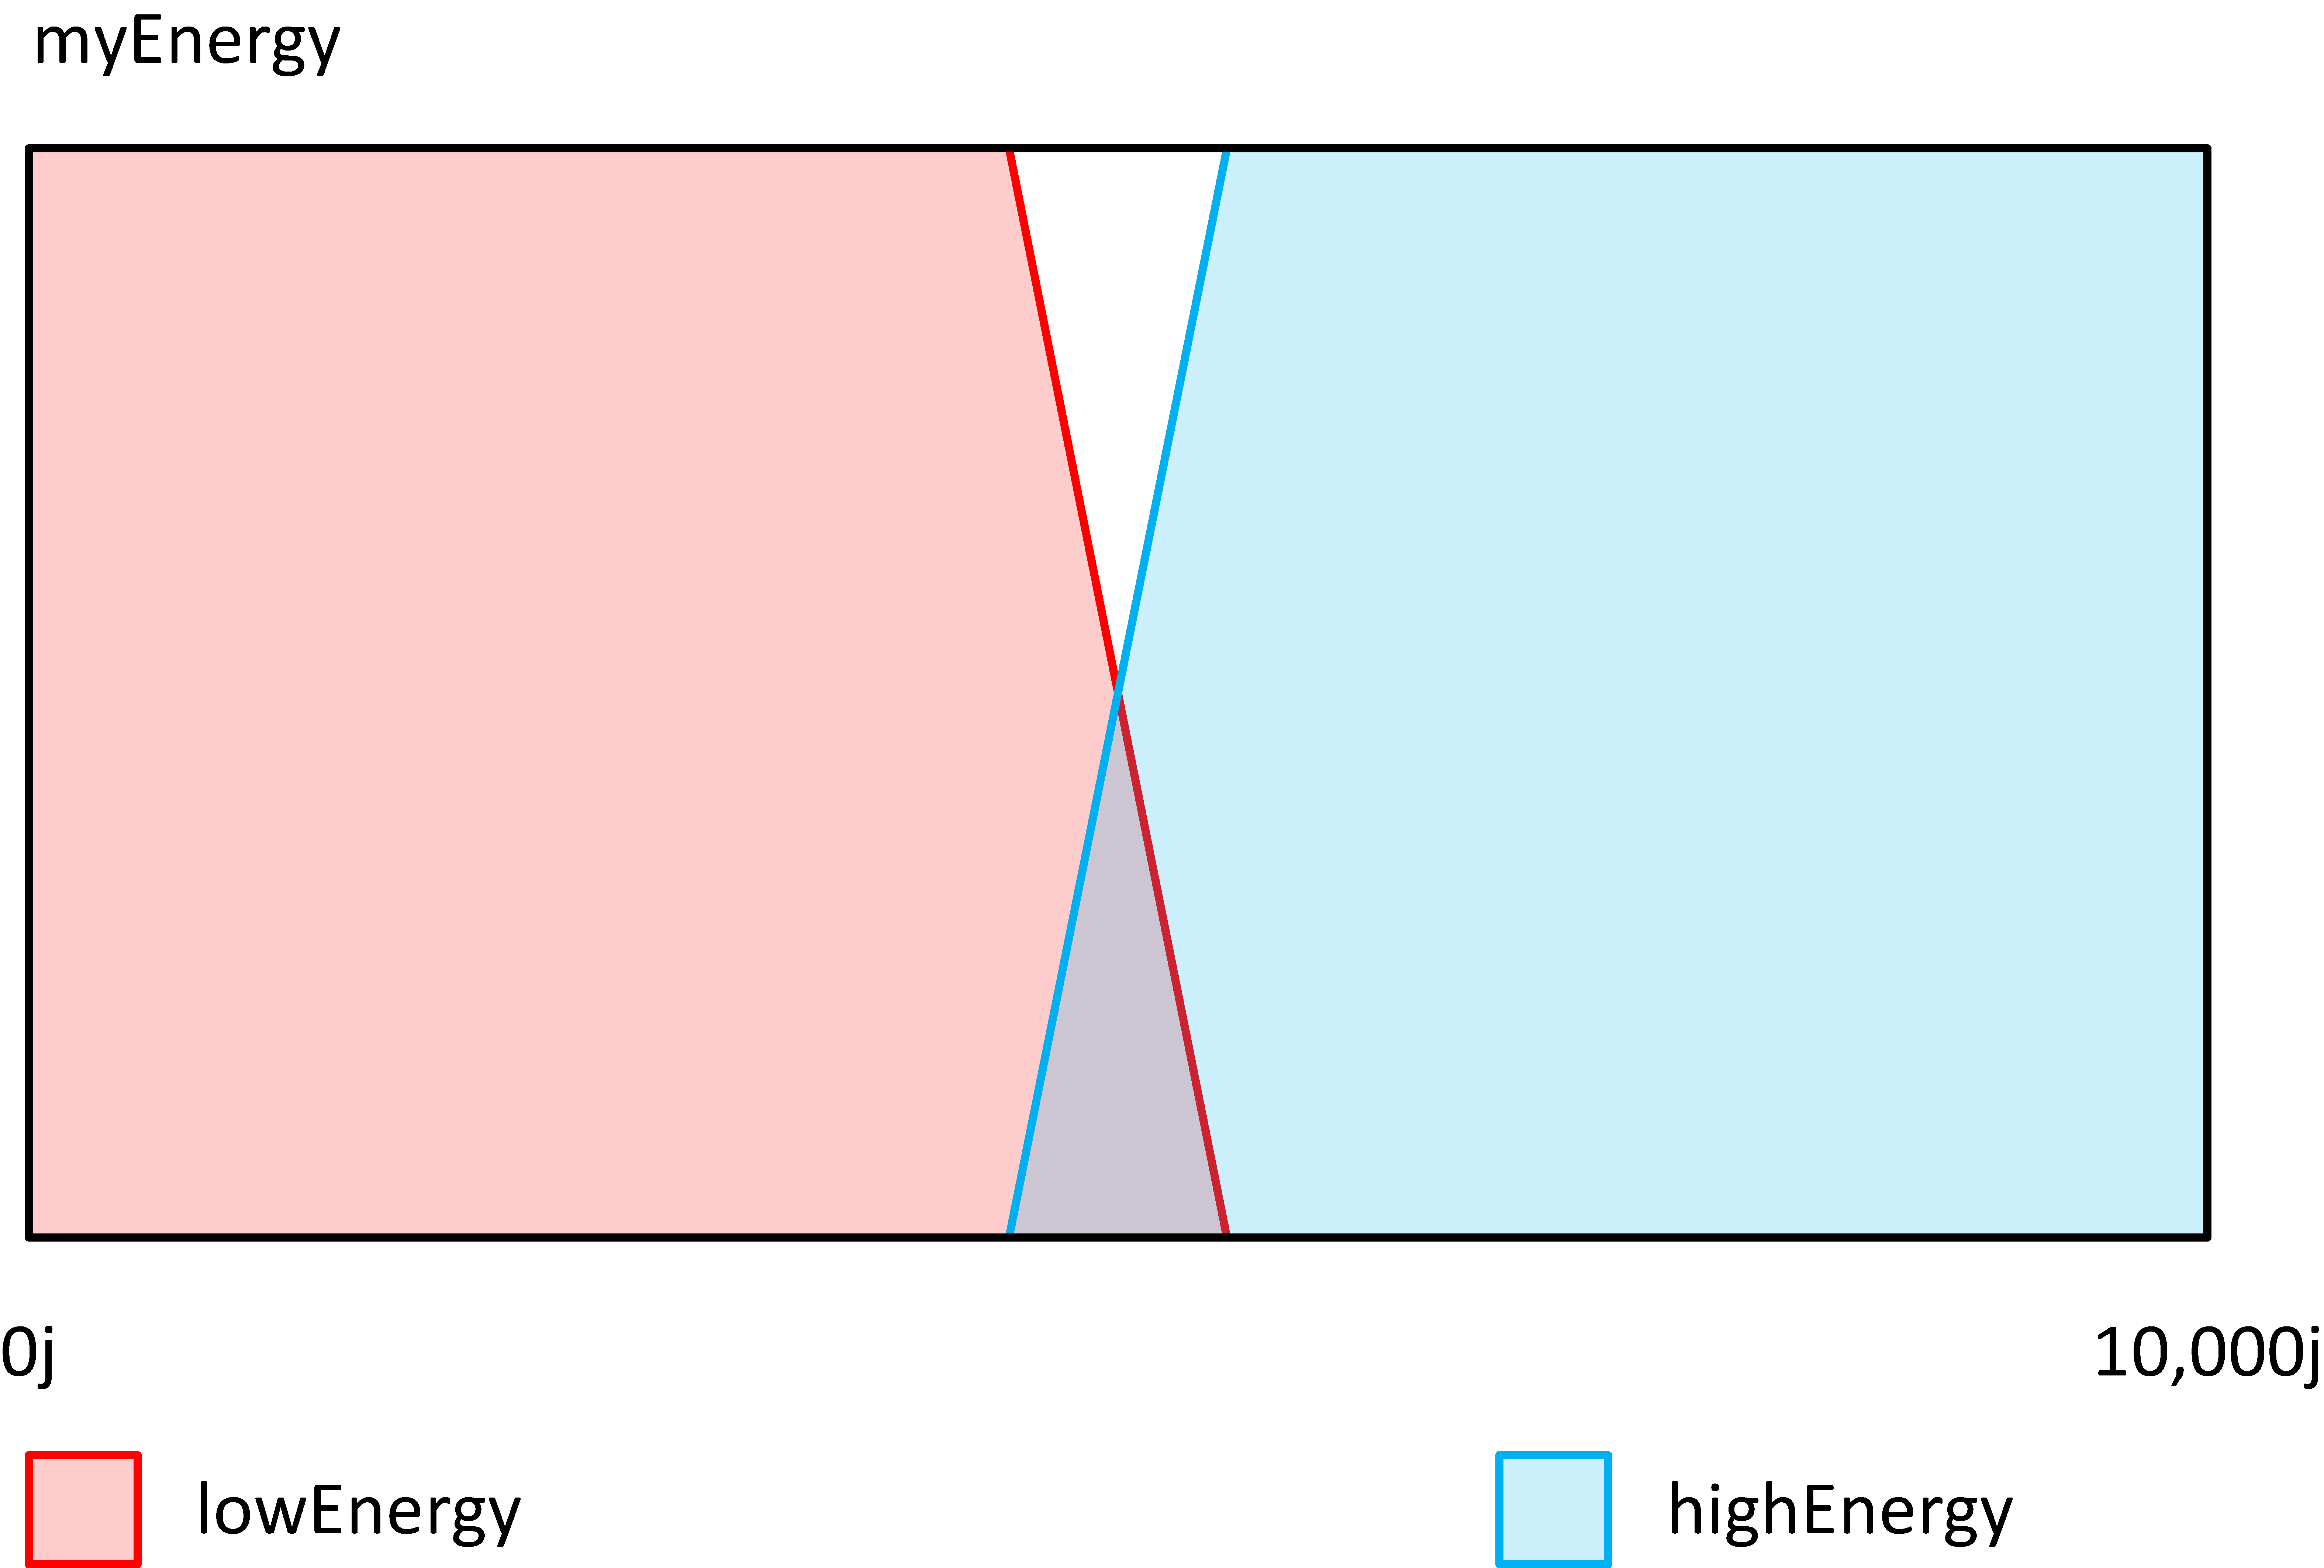
\includegraphics[scale=0.08]{./img/pdf/myEnergySets.pdf}
\end{figure}

\subsection{Target variables}

The sensor returns a list of all the enemy saucers currently in the battle space. This controller only considers the closest saucer as the target, and ignores all other saucers in the list.

\subsubsection{targetDist}

The linguistic variable \emph{targetDist} is the distance from the player to the target. The universe of disclosure for \emph{targetDist} is between 0m and 4802.3m, and the fuzzy sets are defined as \emph{close}, \emph{near}, and \emph{far}.

\begin{figure}[H]
\centering
\caption{\emph{targetDist} fuzzy sets}
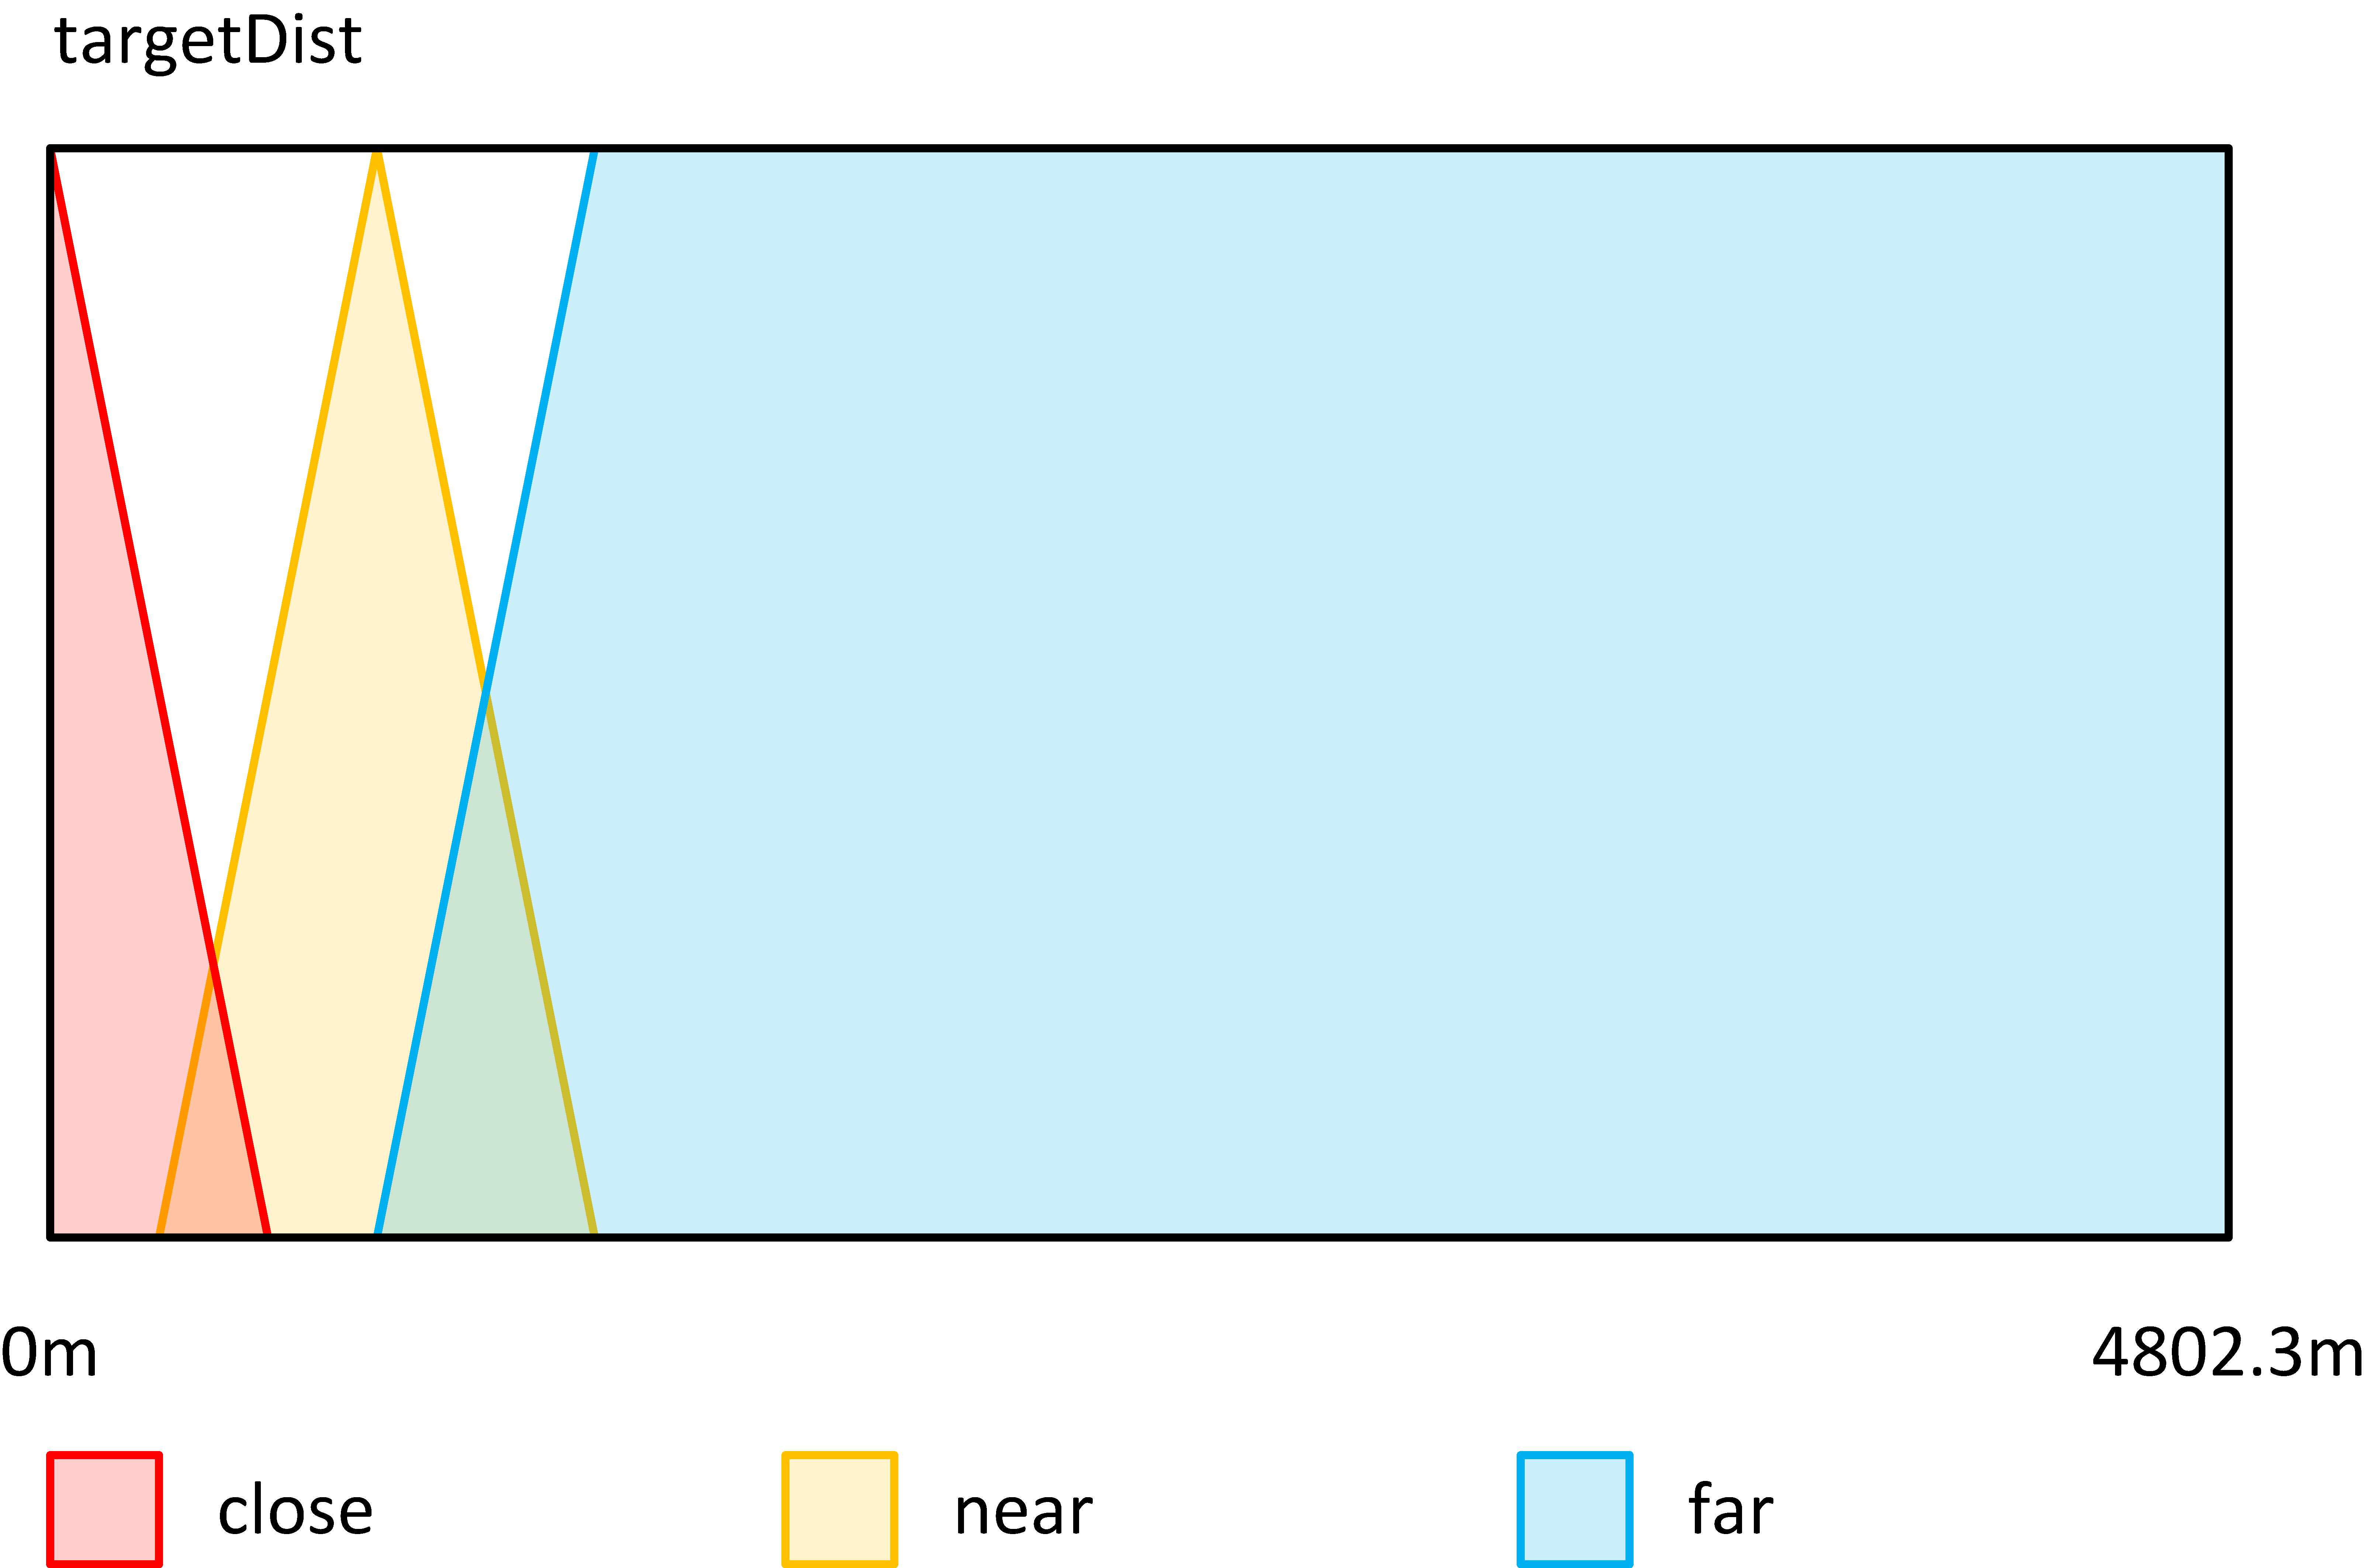
\includegraphics[scale=0.08]{./img/pdf/targetDistSets.pdf}
\end{figure}

\subsubsection{targetAspect}

The linguistic variable \emph{targetAspect} is the direction of the target in relation to the player. The universe of disclosure for \emph{targetAspect} is between -360$^{\circ}$ and +360$^{\circ}$. Positive values rotate to the left, and negative values rotate to the right. The fuzzy sets selected relate to clock positions, similar to what fighter pilots might call out in combat. There are three twelve o'clock positions due to the two revolutions between -360$^{\circ}$ and +360$^{\circ}$.

\begin{figure}[H]
\centering
\caption{\emph{targetAspect} fuzzy sets}
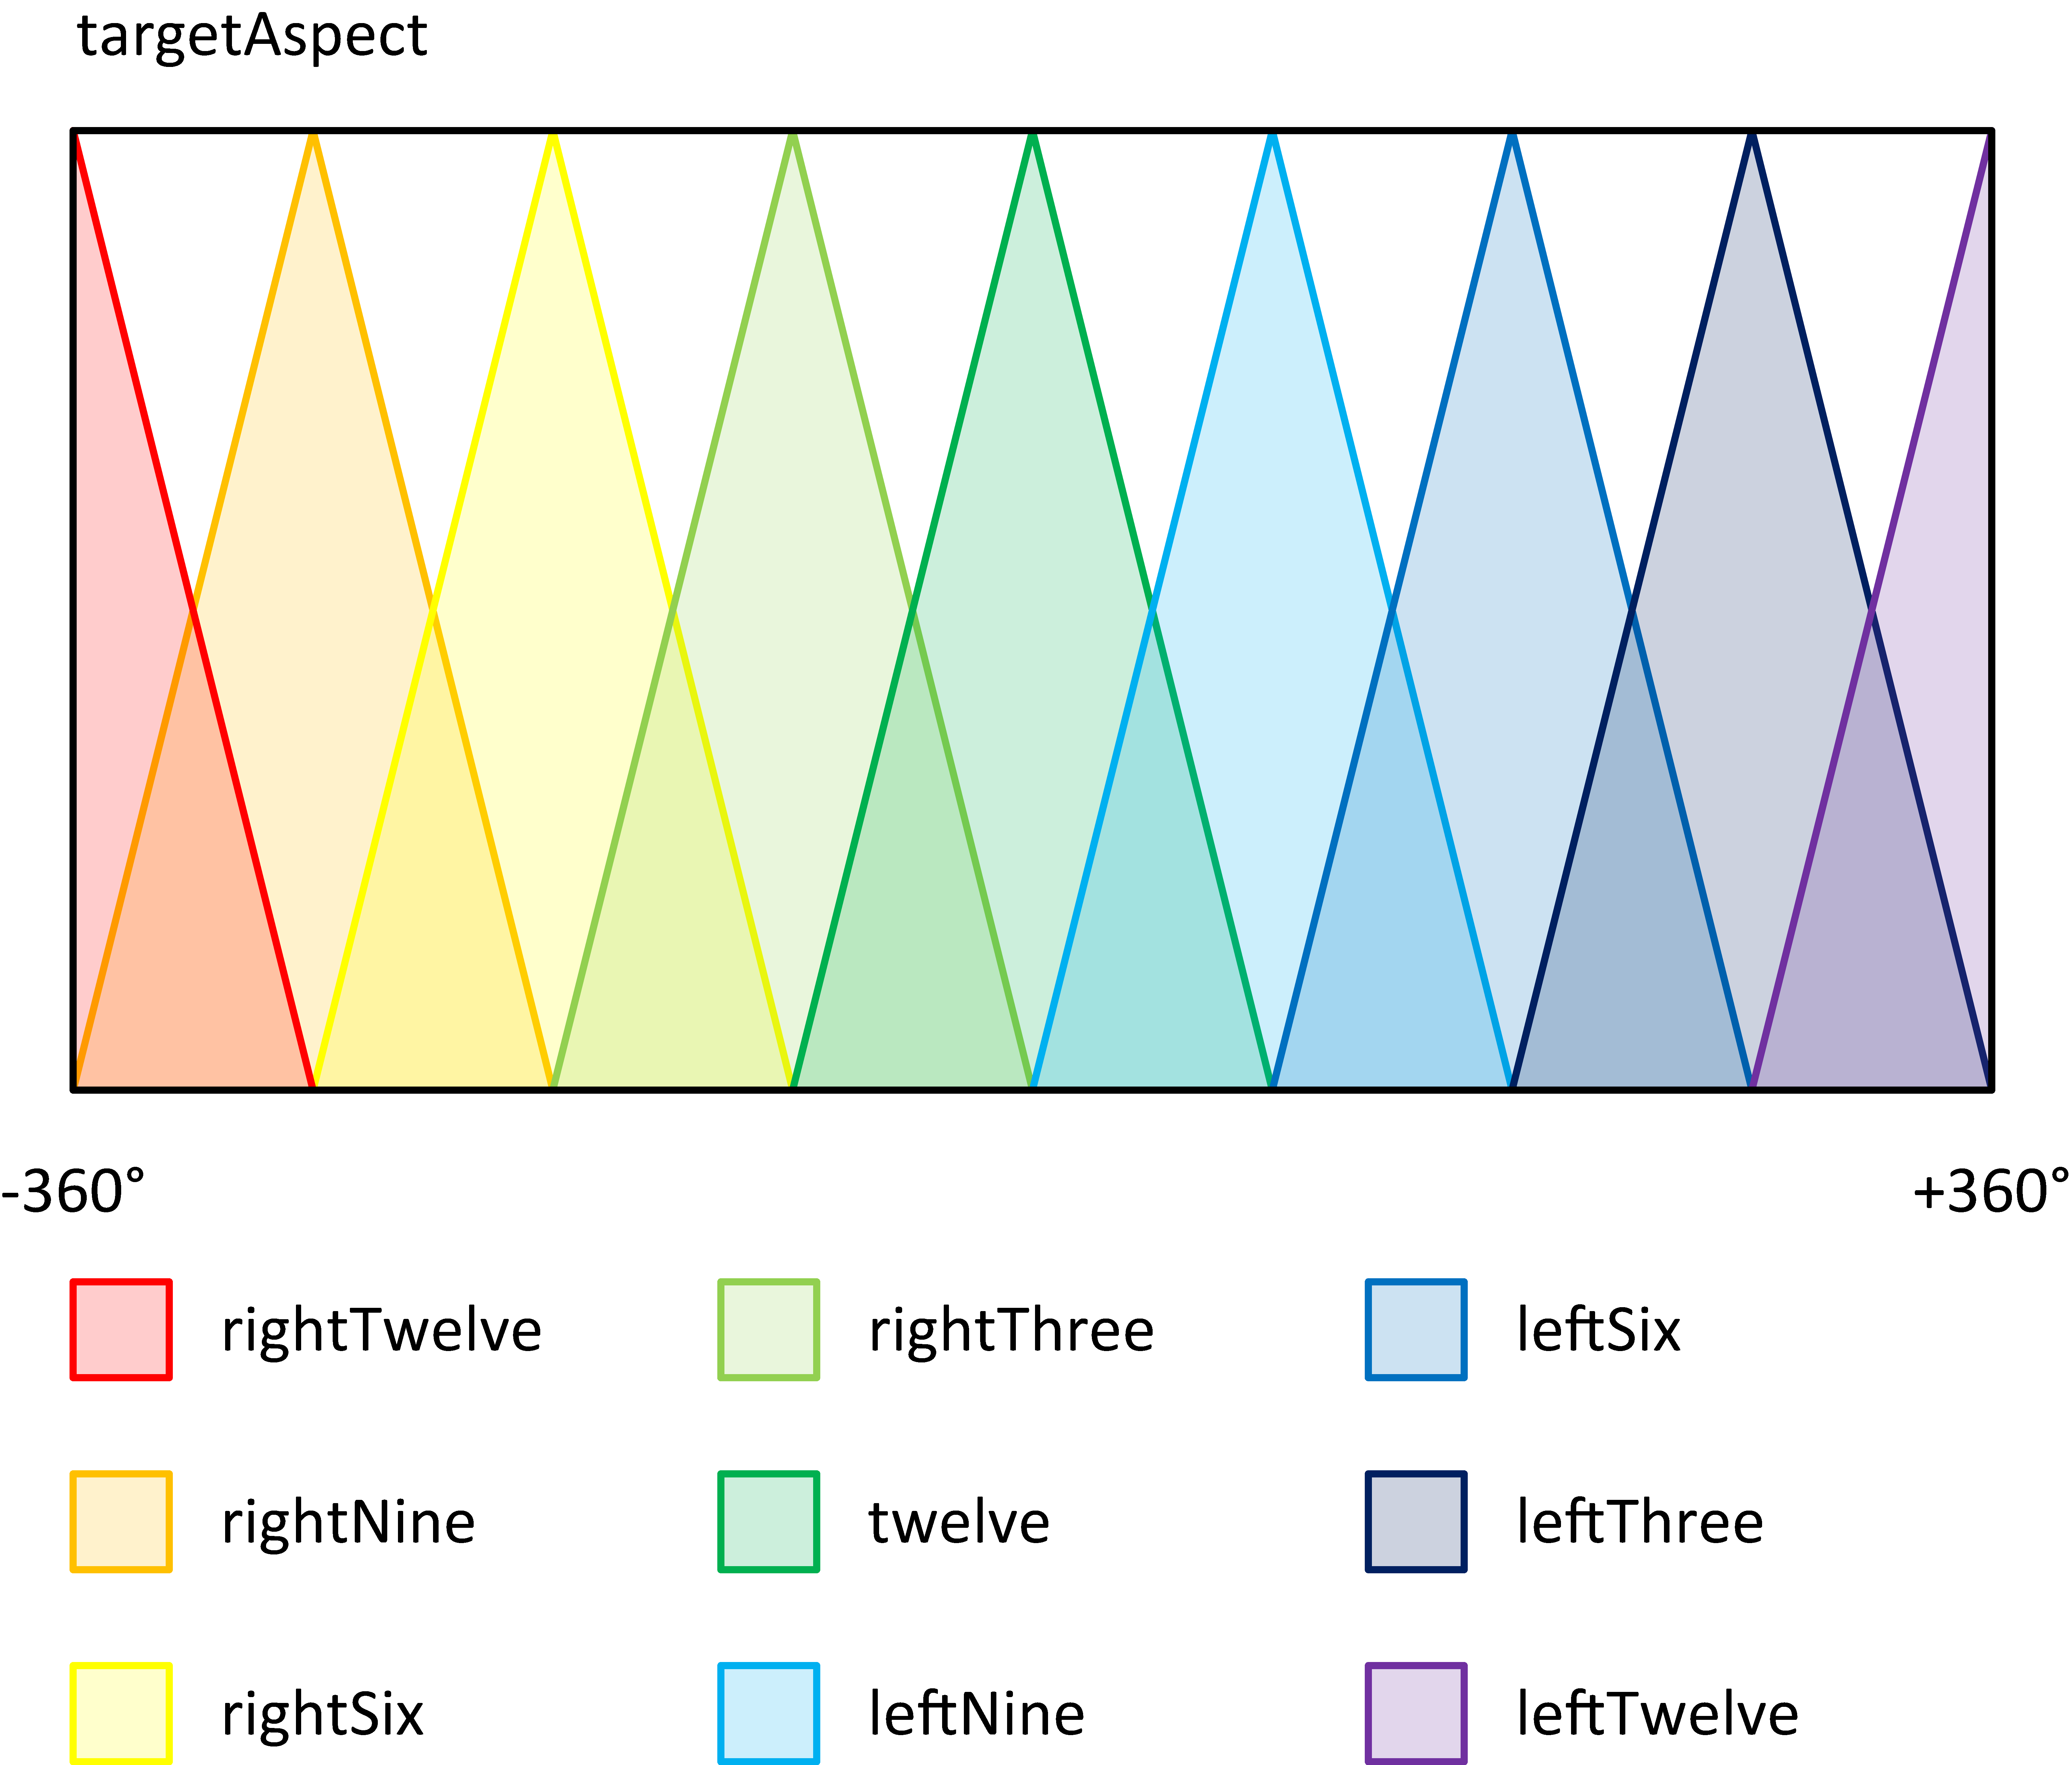
\includegraphics[scale=0.08]{./img/pdf/targetAspectSets.pdf}
\end{figure}

\subsubsection{targetAngleOff}

The linguistic variable \emph{targetAngleOff} relates to the target's current heading, in relation to the player's current heading. For example, if the target is heading towards the player perpendicularly from the right, the target's angle-off would be +90$^{\circ}$. Similarly, if the target has the exact same heading as the player, the target's angle-off would be 0$^{\circ}$. Again, positive values rotate to the left, and negative values rotate to the right. The universe of disclosure is between -360$^{\circ}$ and +360$^{\circ}$. The fuzzy sets selected mimic clock positions, similar to \emph{targetAspect}, however are named with degree values. A merge is when the player and target have opposite angle-off's, ie. 180$^{\circ}$. In this situation, if the player and target were in front of each other, they would facing each other, and would be about to directly pass each other, in a ``merge''.

\begin{figure}[H]
\centering
\caption{\emph{targetAngleOff} fuzzy sets}
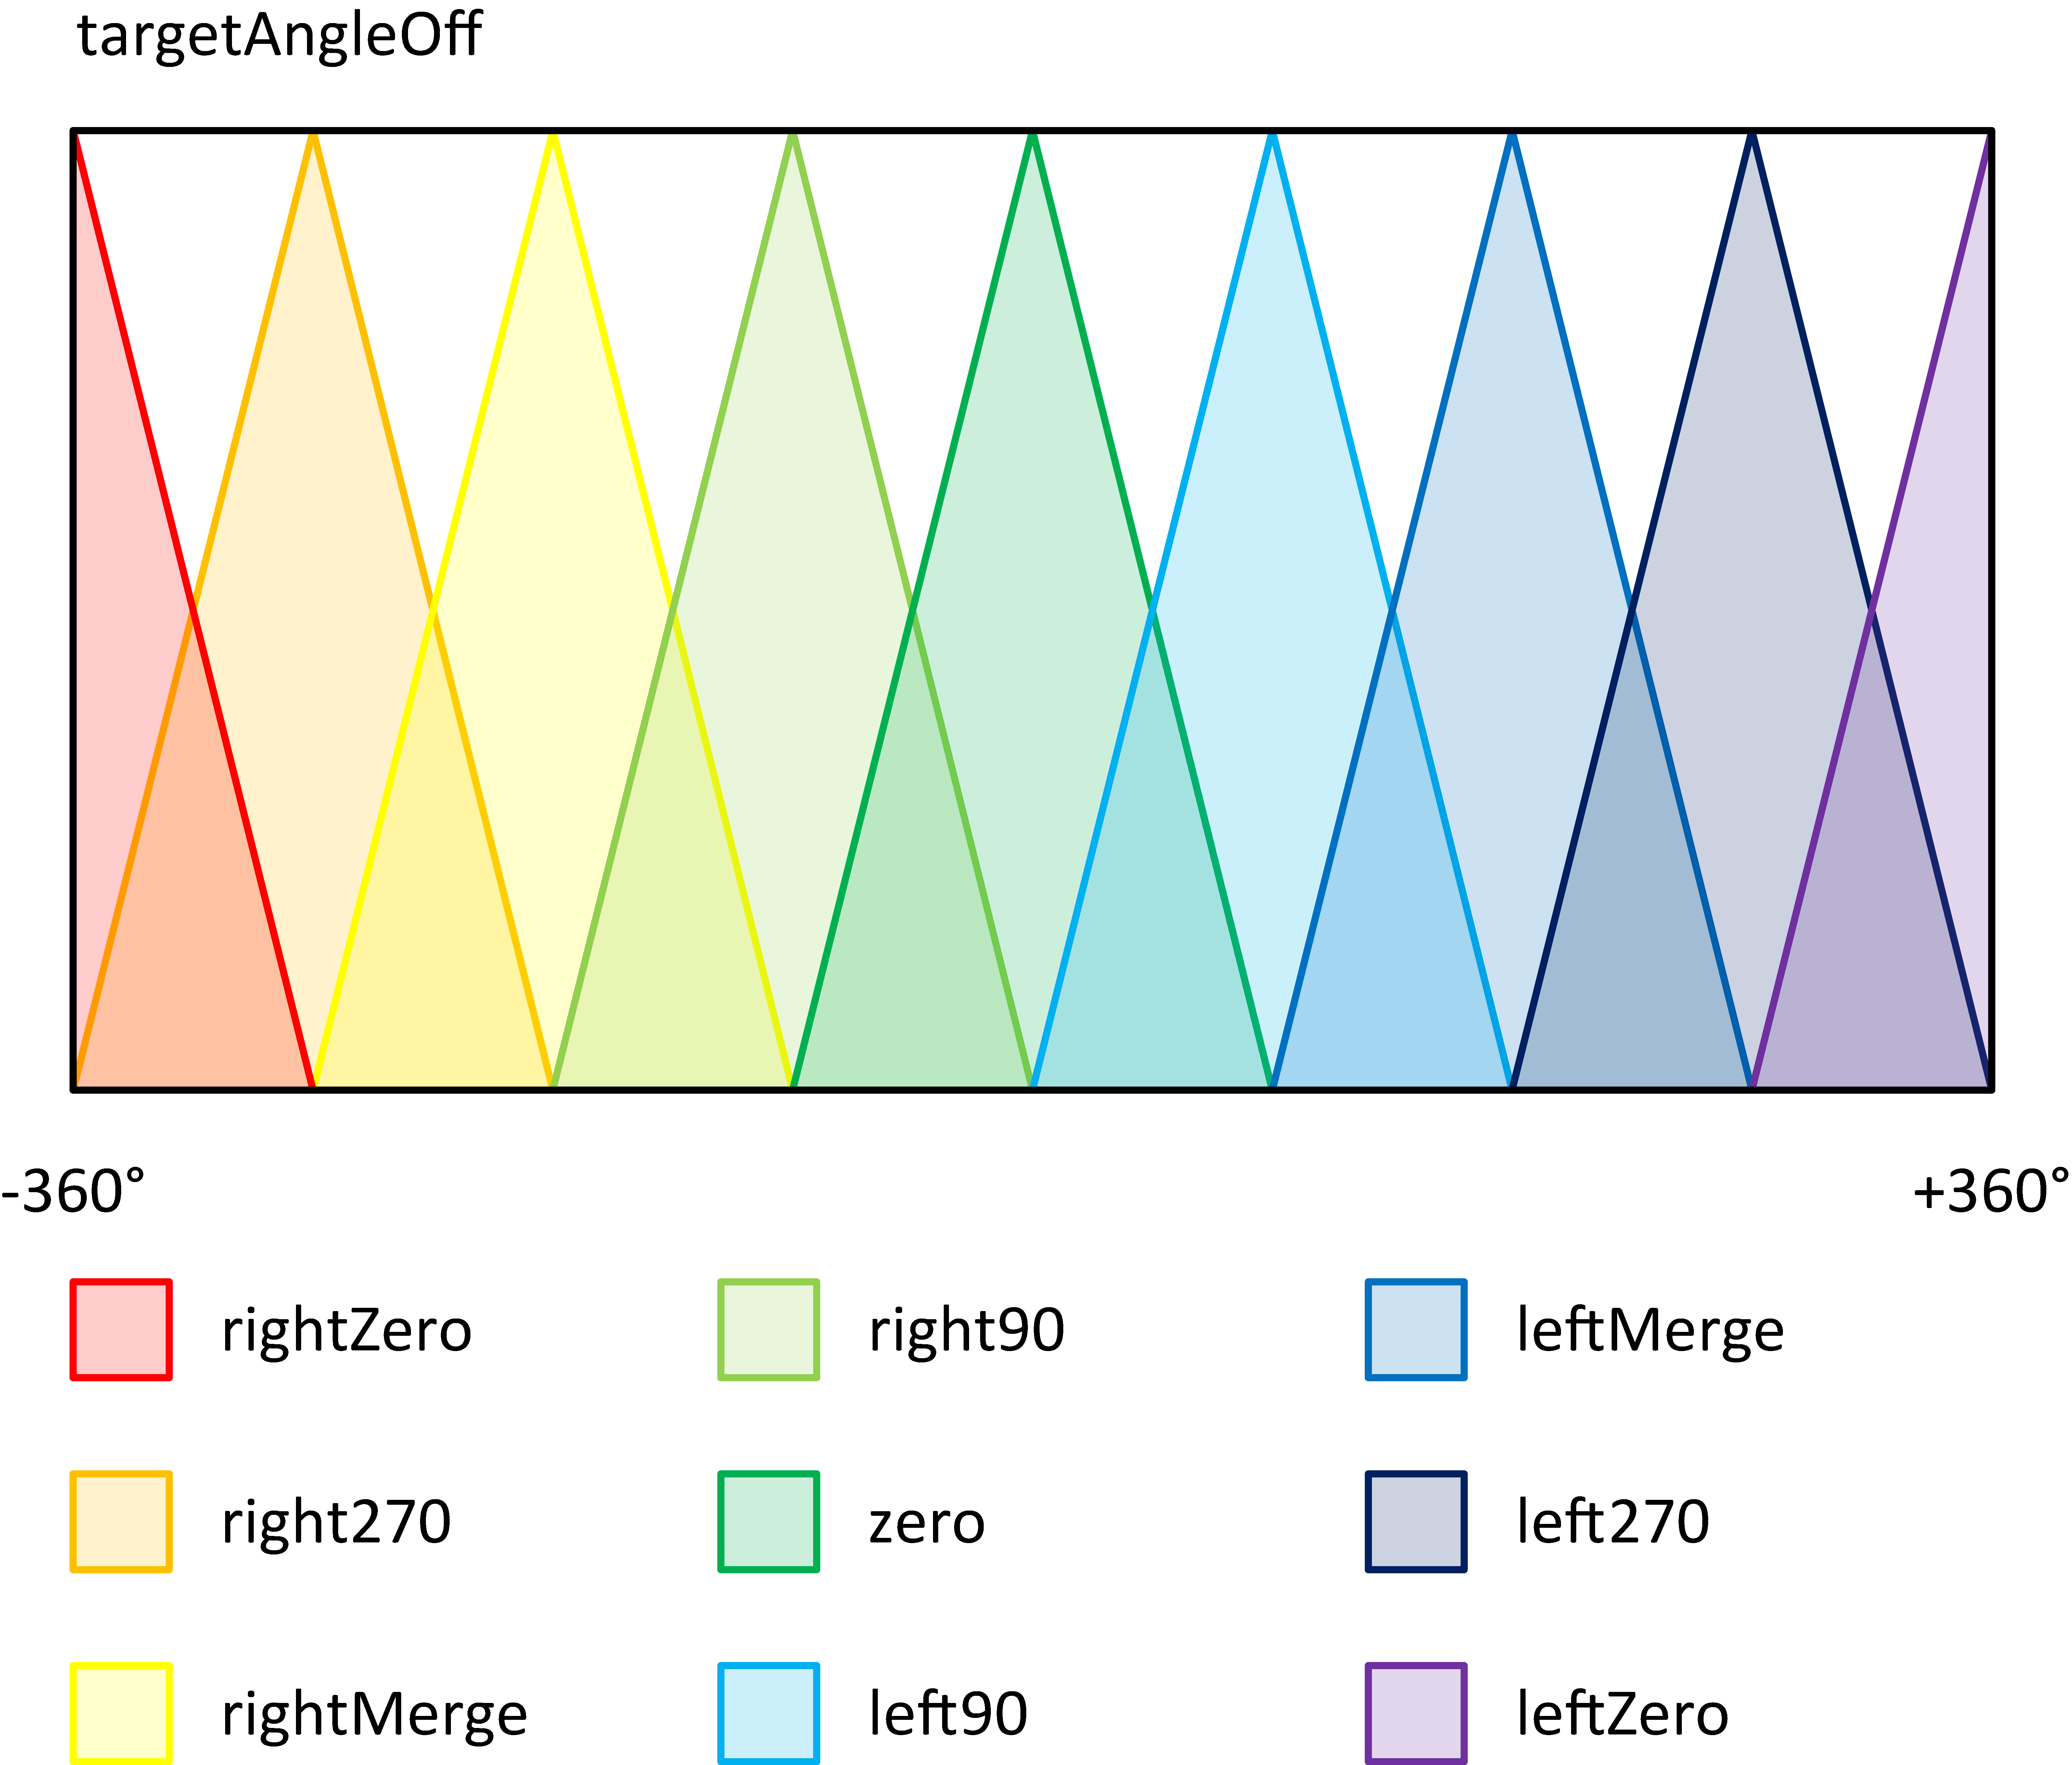
\includegraphics[scale=0.08]{./img/pdf/targetAngleOffSets.pdf}
\end{figure}

\subsubsection{targetEnergyDiff}

The linguistic variable \emph{targetEnergyDiff} relates to the difference between the player's energy and the current target's energy. The universe of disclosure for \emph{targetEnergyDiff} is between -10,000j and +10,000j. The fuzzy sets selected for this linguistic variable are \emph{losing} and \emph{winning}.

\begin{figure}[H]
\centering
\caption{\emph{targetEnergyDiff} fuzzy sets}
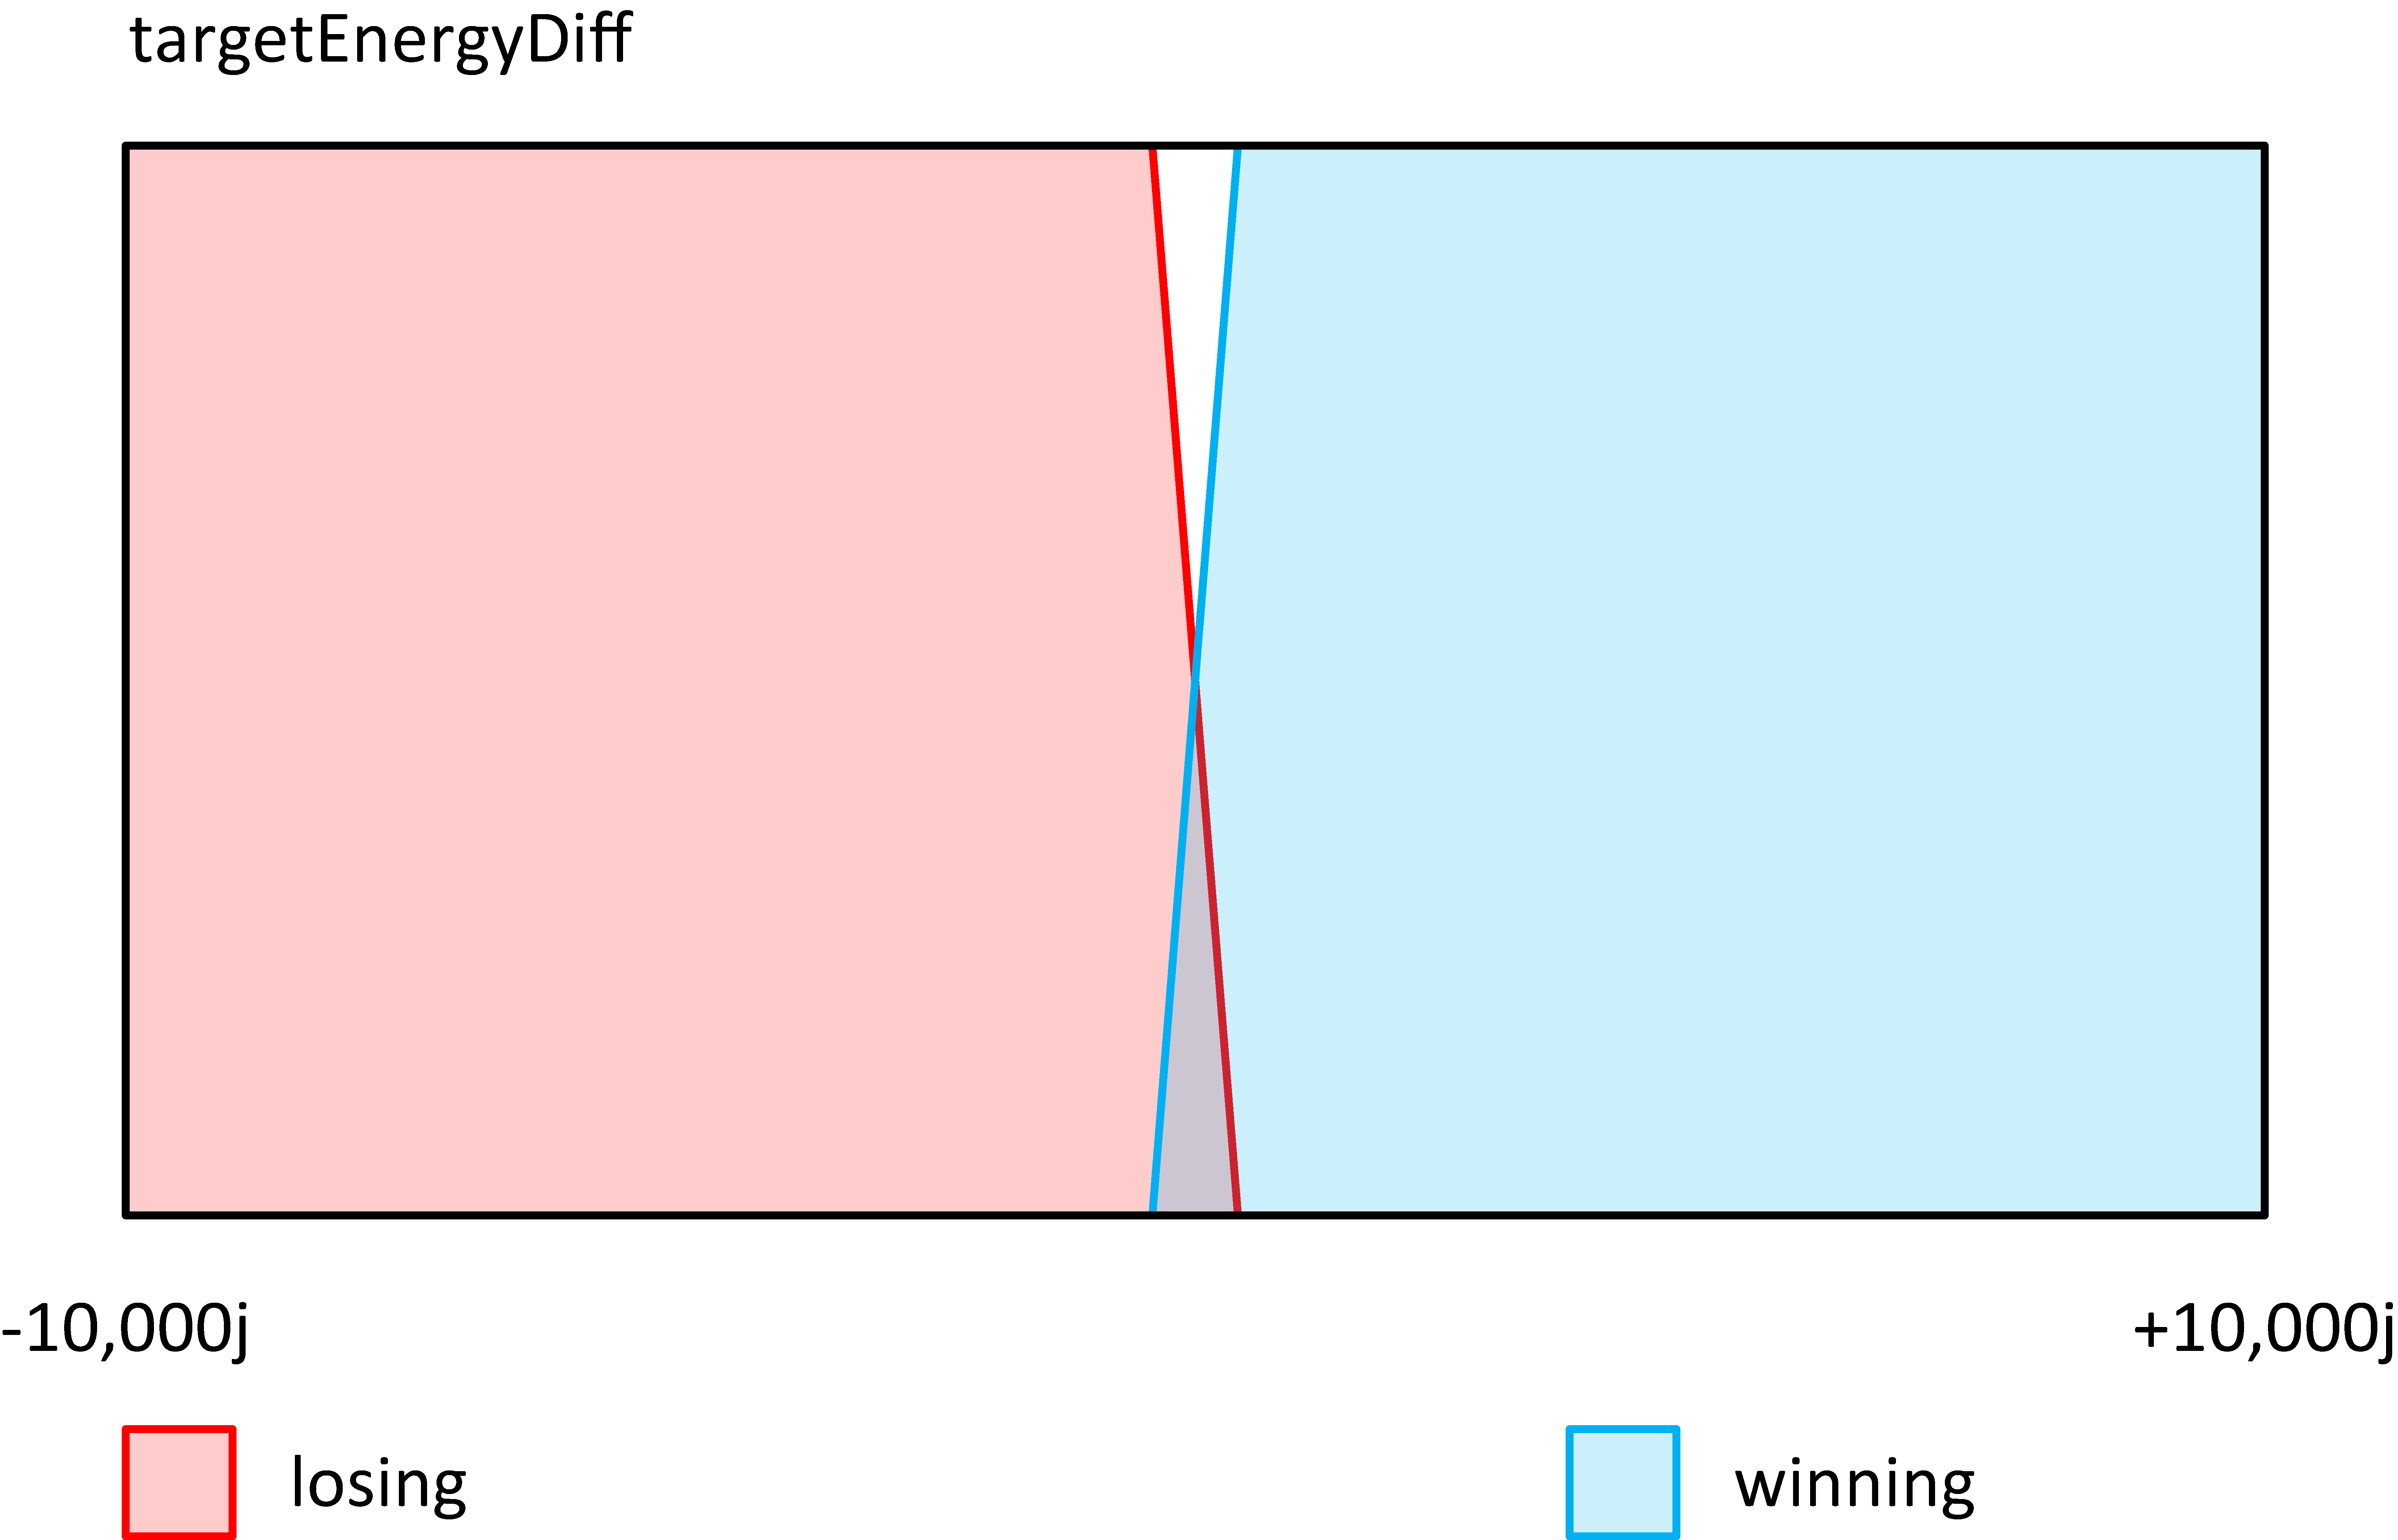
\includegraphics[scale=0.08]{./img/pdf/targetEnergyDiffSets.pdf}
\end{figure}

\subsection{Blast variables}

The sensor returns a list of all energy blasts currently in the battle space. This controller only considers the closest energy blast to dodge, and ignores all other blasts in the list.

\subsubsection{blastDist}

The linguistic variable \emph{blastDist} is the distance from the player to the energy blast. The universe of disclosure for \emph{blastDist} is between 0m and 4802.3m, and the fuzzy sets are defined as \emph{close} and \emph{far}.

\begin{figure}[H]
\centering
\caption{\emph{blastDist} fuzzy sets}
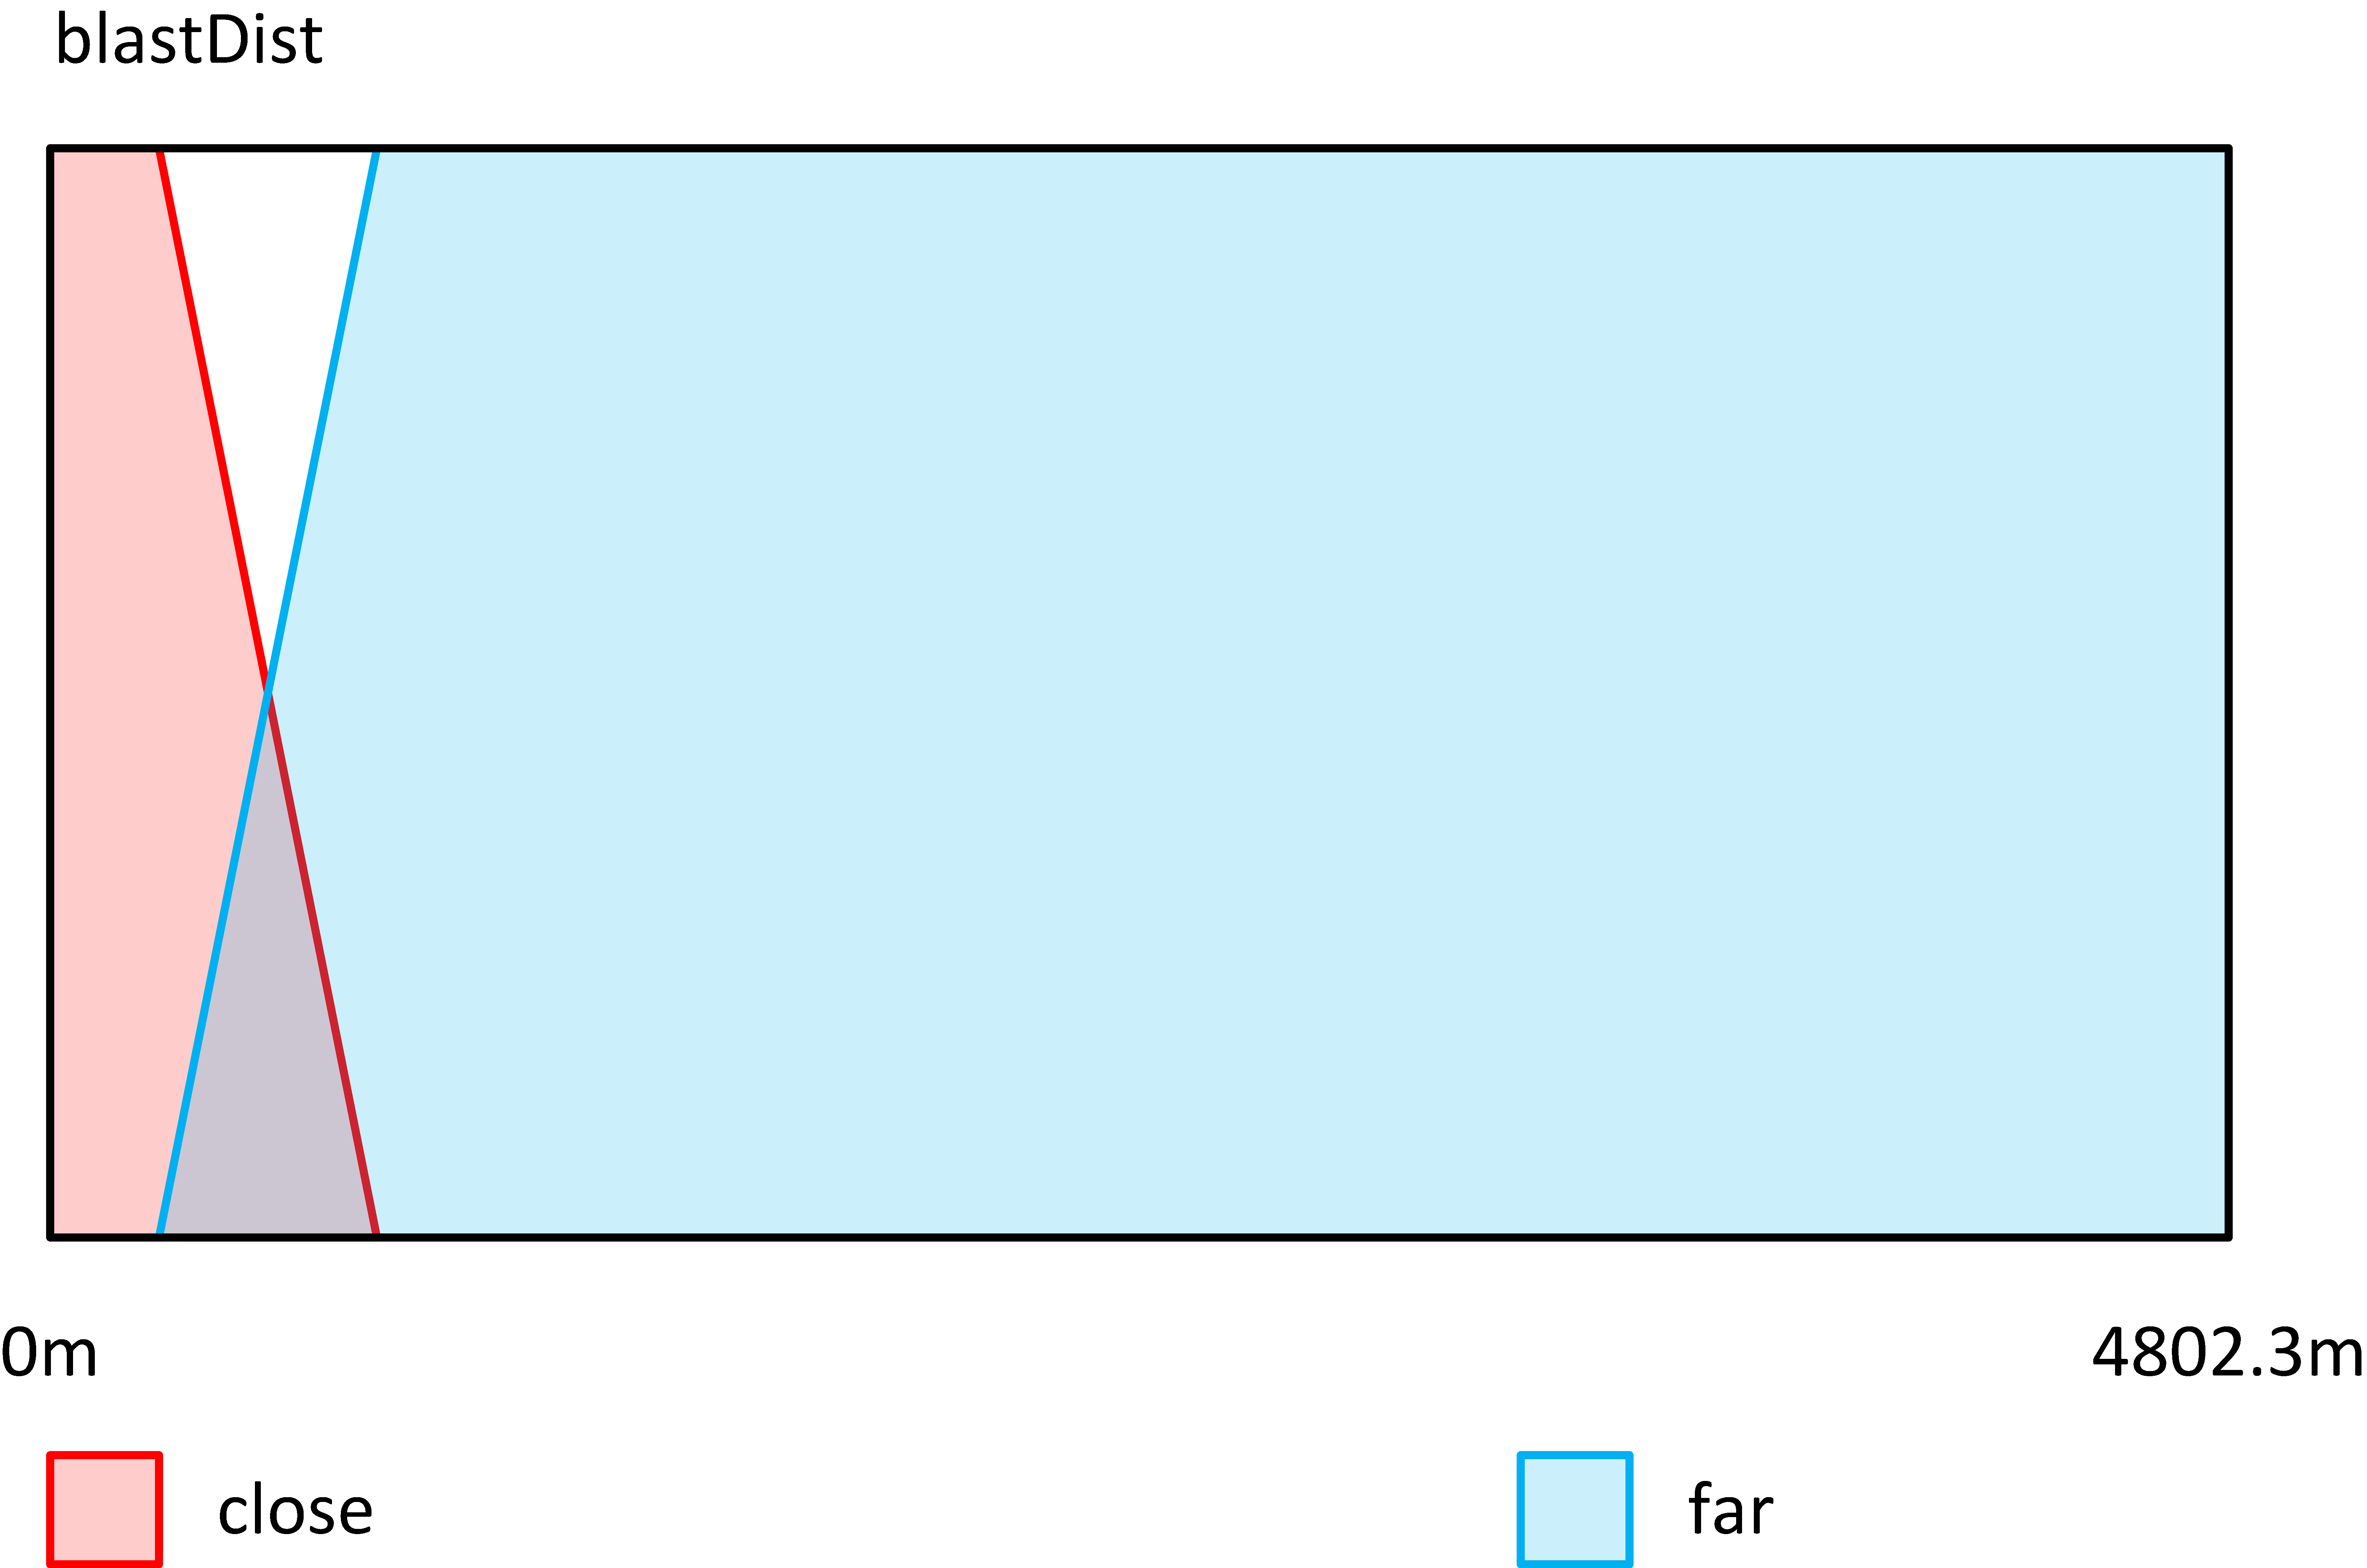
\includegraphics[scale=0.08]{./img/pdf/blastDistSets.pdf}
\end{figure}

\subsubsection{blastAspect}

The linguistic variable \emph{blastAspect} is similar to \emph{targetAspect}, but relates to the direction from the player to the energy blast. Similar fuzzy sets, based on the clock analogy have been used.

\begin{figure}[H]
\centering
\caption{\emph{blastAspect} fuzzy sets}
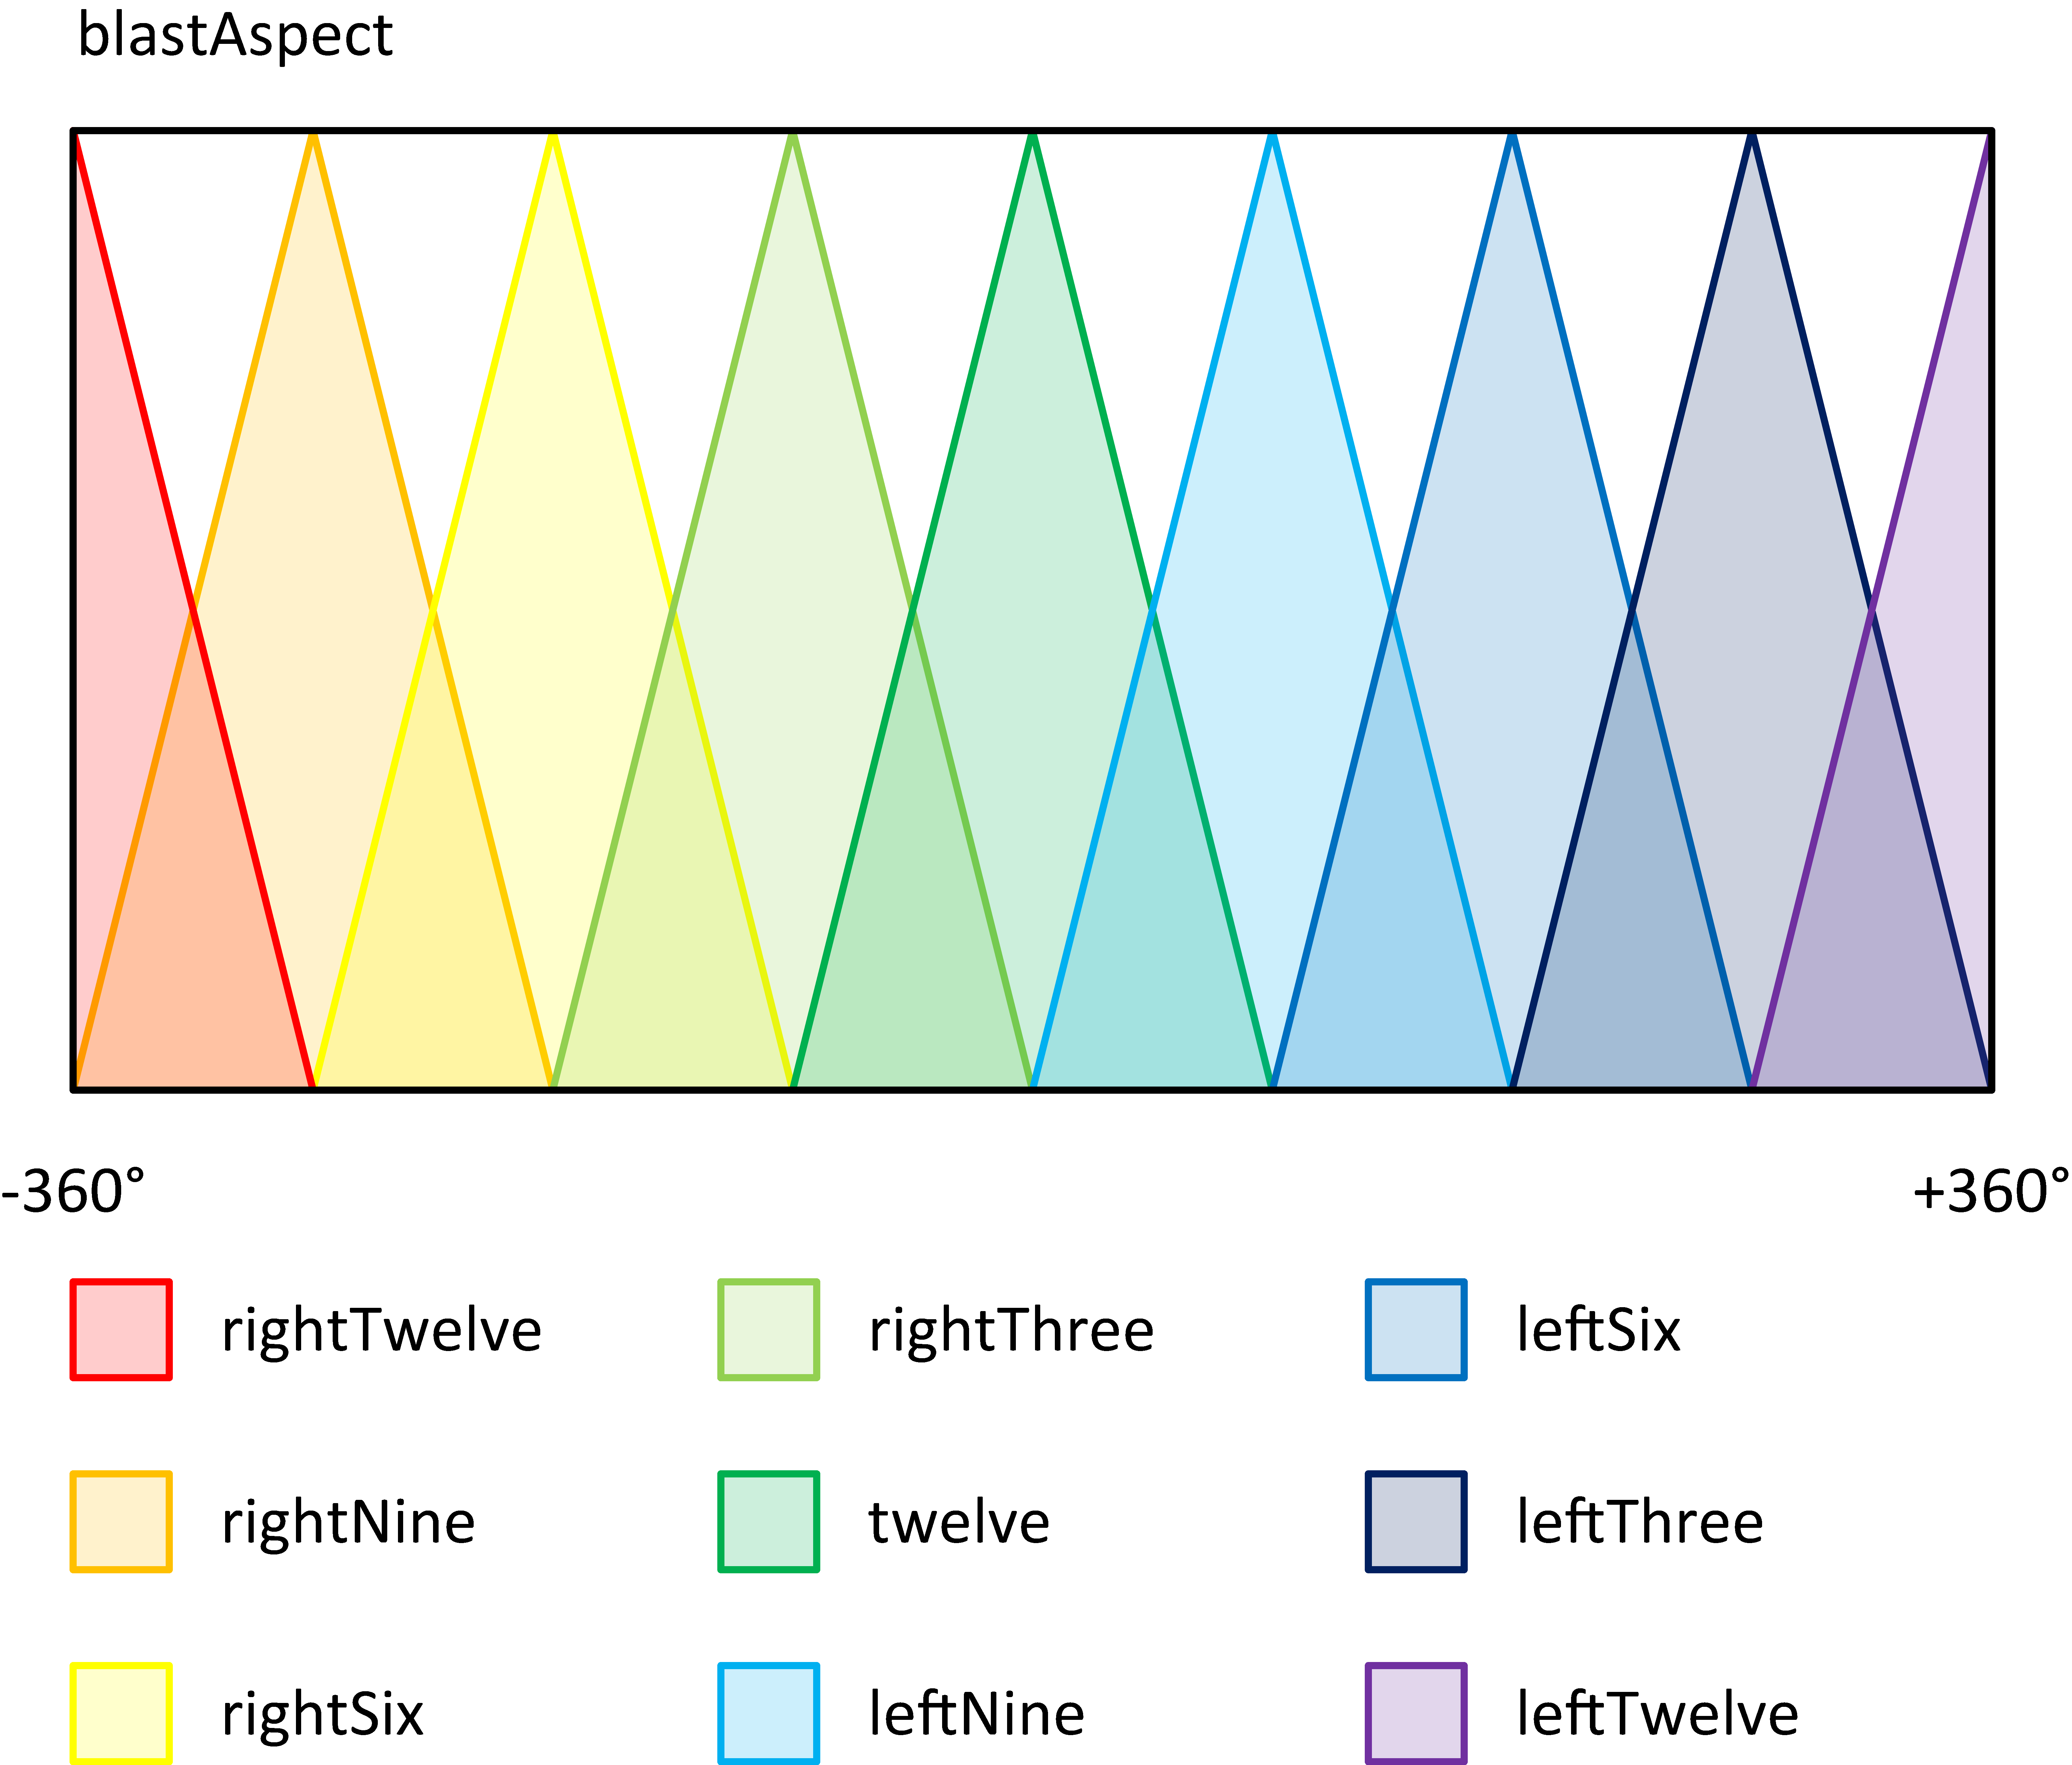
\includegraphics[scale=0.08]{./img/pdf/blastAspectSets.pdf}
\end{figure}

\subsubsection{blastAngleOff}

The linguistic variable \emph{blastAngleOff} is similar to \emph{targetAngleOff}, but references the current heading of the energy blast in relation to the player's heading. Similar fuzzy sets have also been used.

\begin{figure}[H]
\centering
\caption{\emph{blastAngleOff} fuzzy sets}
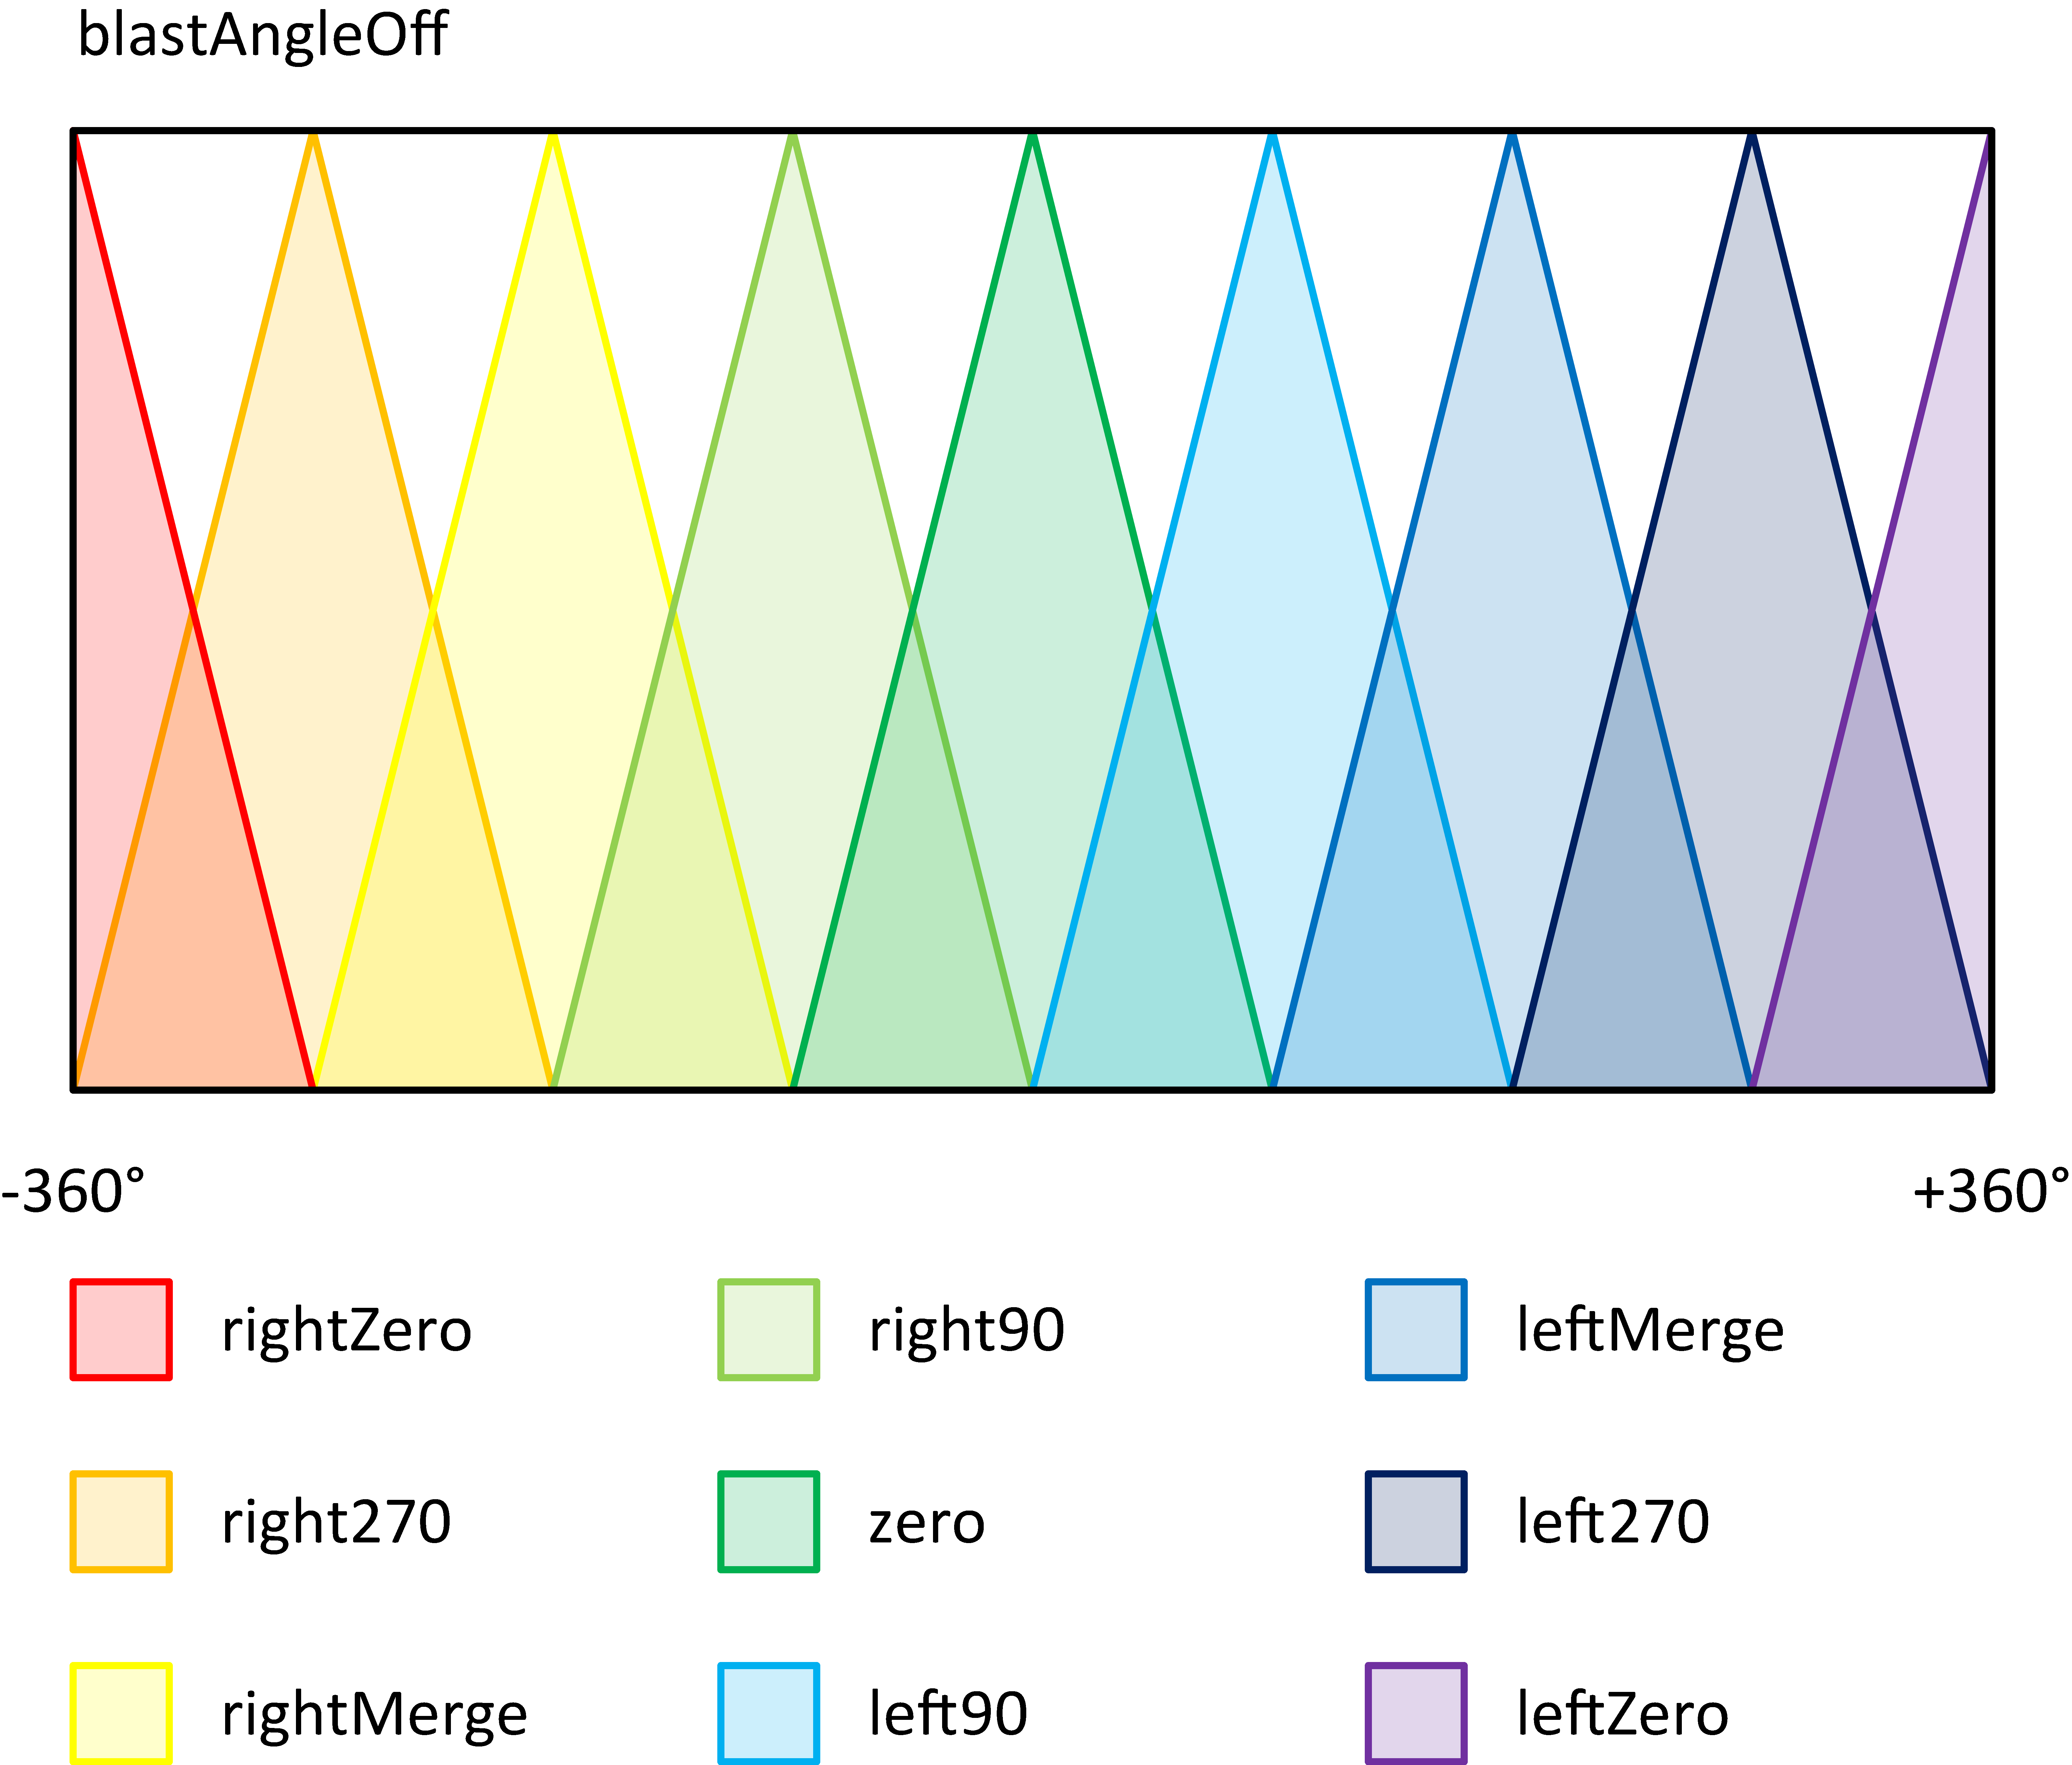
\includegraphics[scale=0.08]{./img/pdf/blastAngleOffSets.pdf}
\end{figure}

\subsection{Powerup variables}

The sensor returns a list of all powerups that currently exist in the battle space. To conserve energy, this controller only reacts to powerups only if they are nearby, and assumes that powerups that are far would most likely be consumed by an enemy by the time the player arrives.

\subsubsection{powerUpDist}

The linguistic variable \emph{powerUpDist} is the distance between the target and the powerup. Similar to \emph{targetDist}, the universe of disclosure is between 0m and 4802.3m. Similar fuzzy sets have also been used.

\begin{figure}[H]
\centering
\caption{\emph{powerUpDist} fuzzy sets}
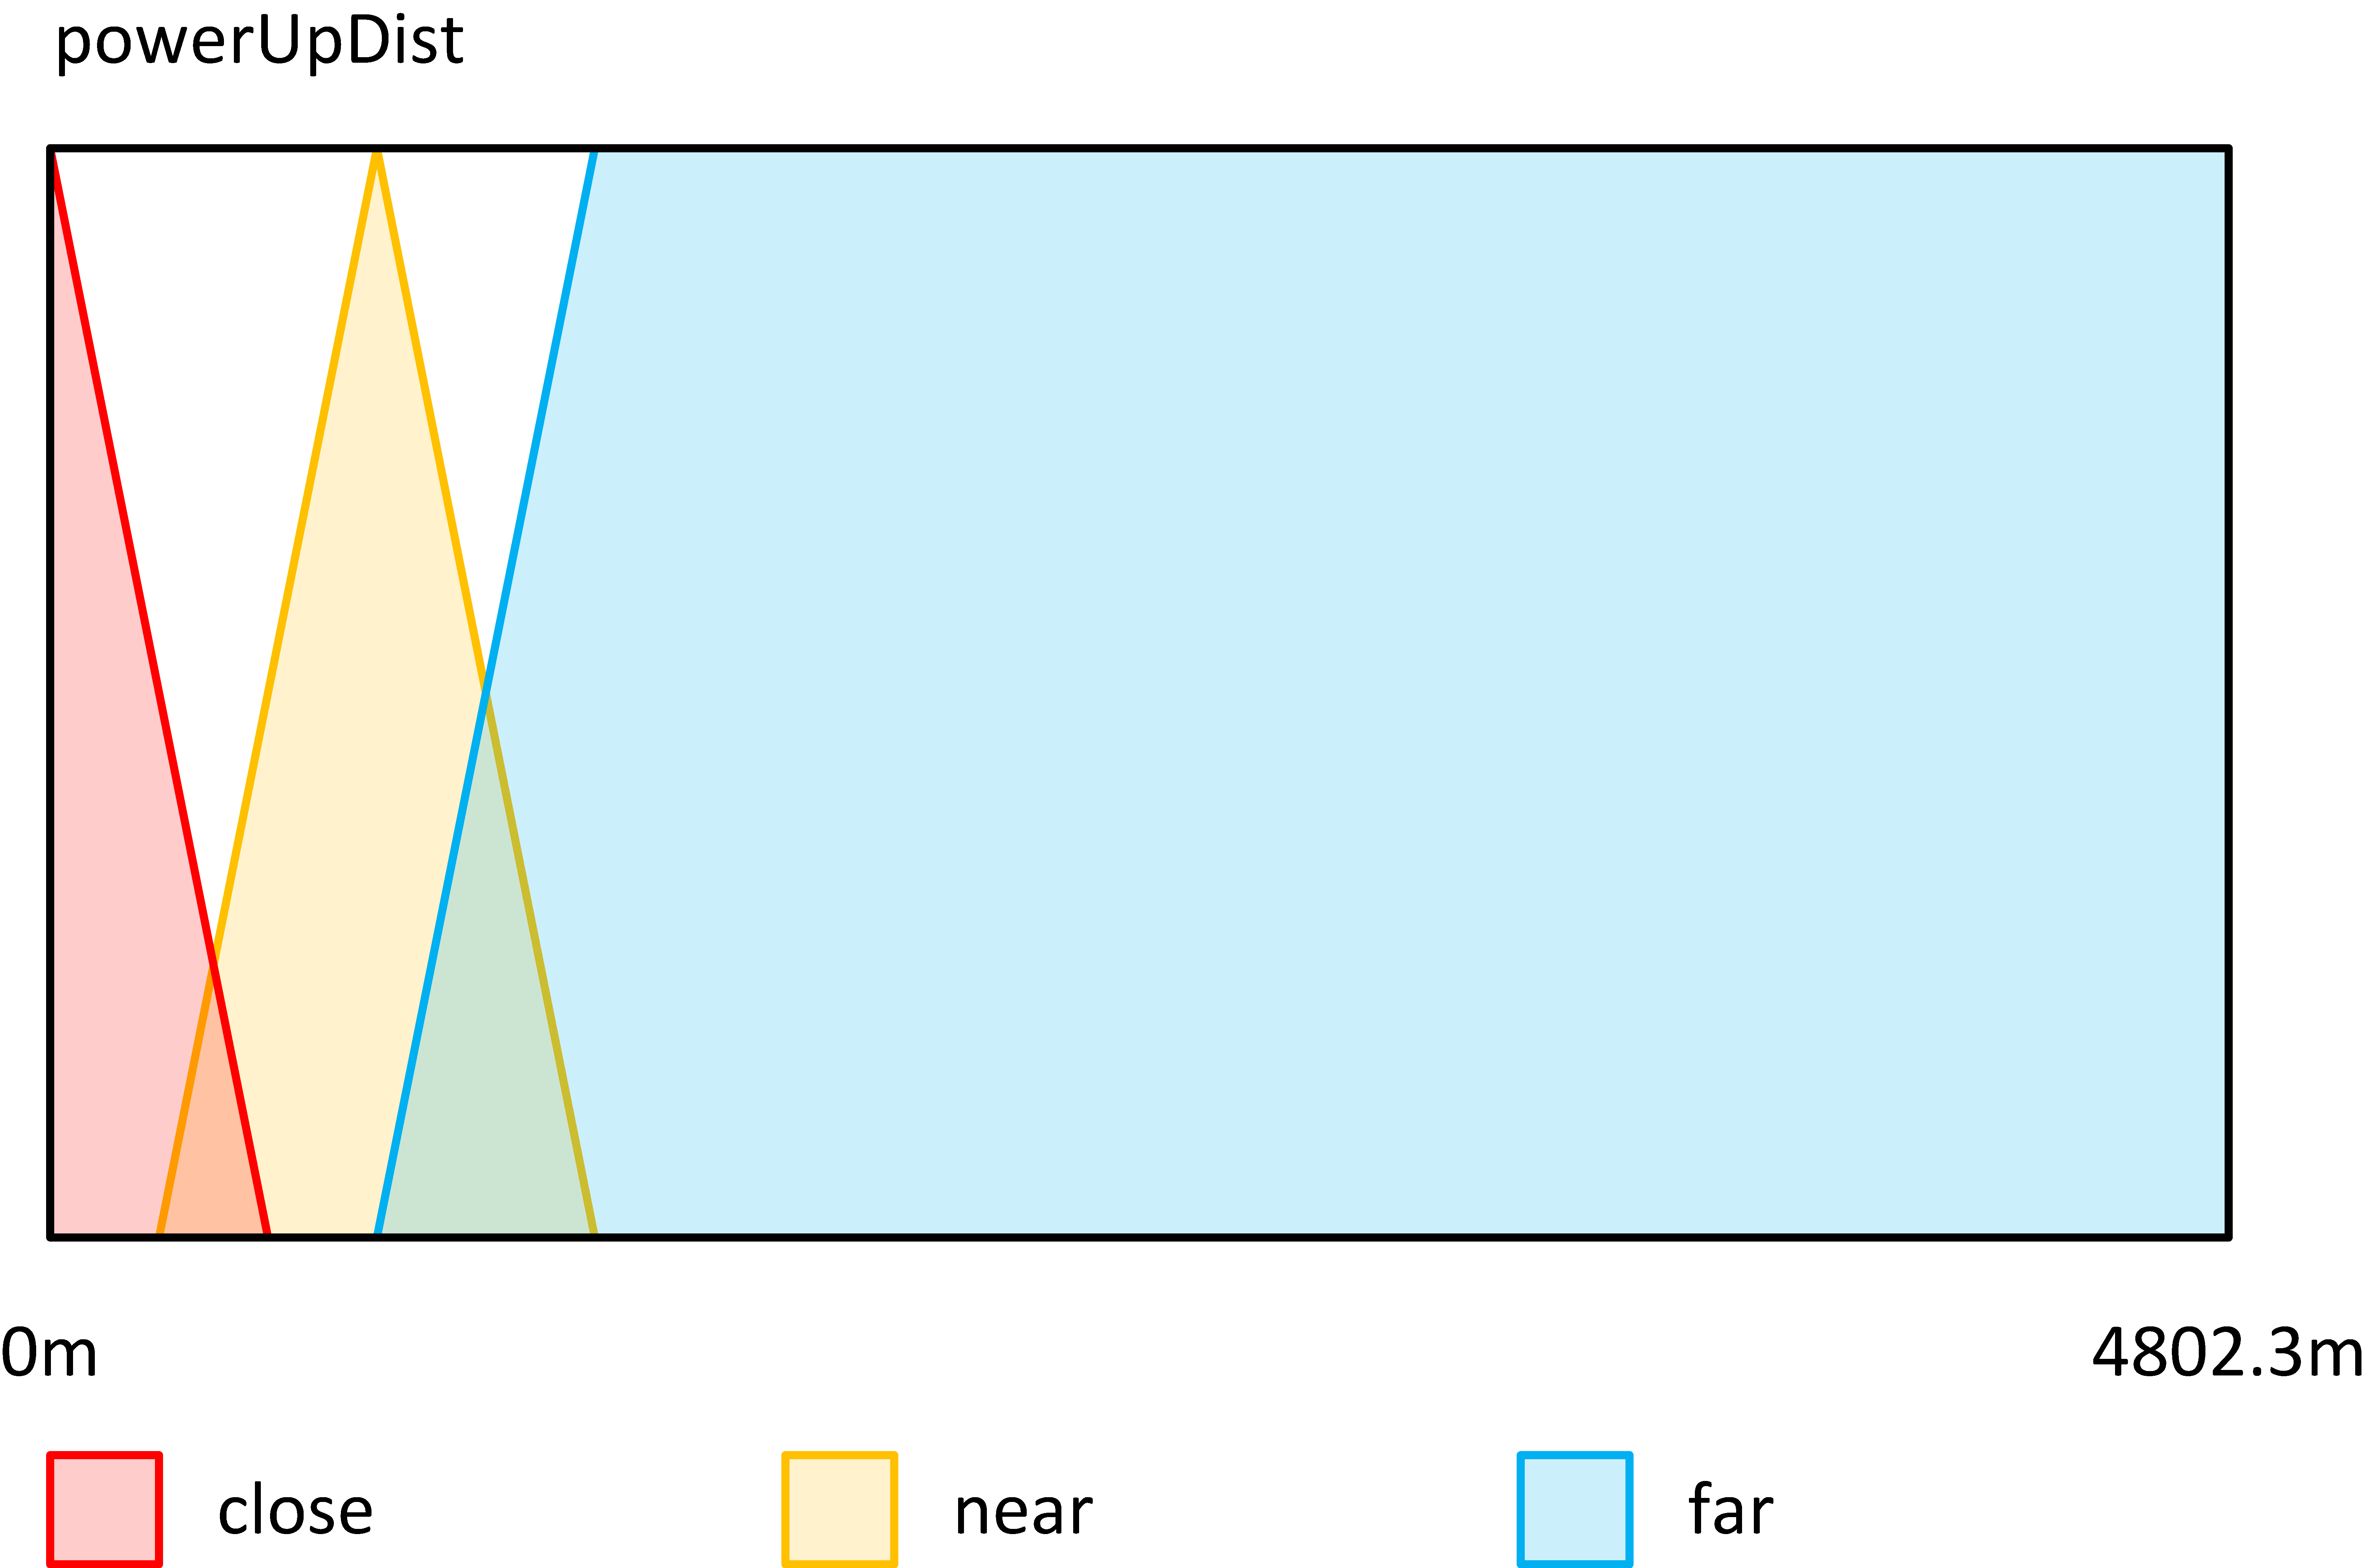
\includegraphics[scale=0.08]{./img/pdf/powerUpDistSets.pdf}
\end{figure}

\subsubsection{powerUpAspect}

The linguistic variable \emph{powerUpAspect} is the direction of the powerup in relation to the player. Again, the clock analogy has been used to determine the fuzzy sets. However, the angle-off of the powerup is not considered, since it is stationary and does not change its heading.

\begin{figure}[H]
\centering
\caption{\emph{powerUpAspect} fuzzy sets}
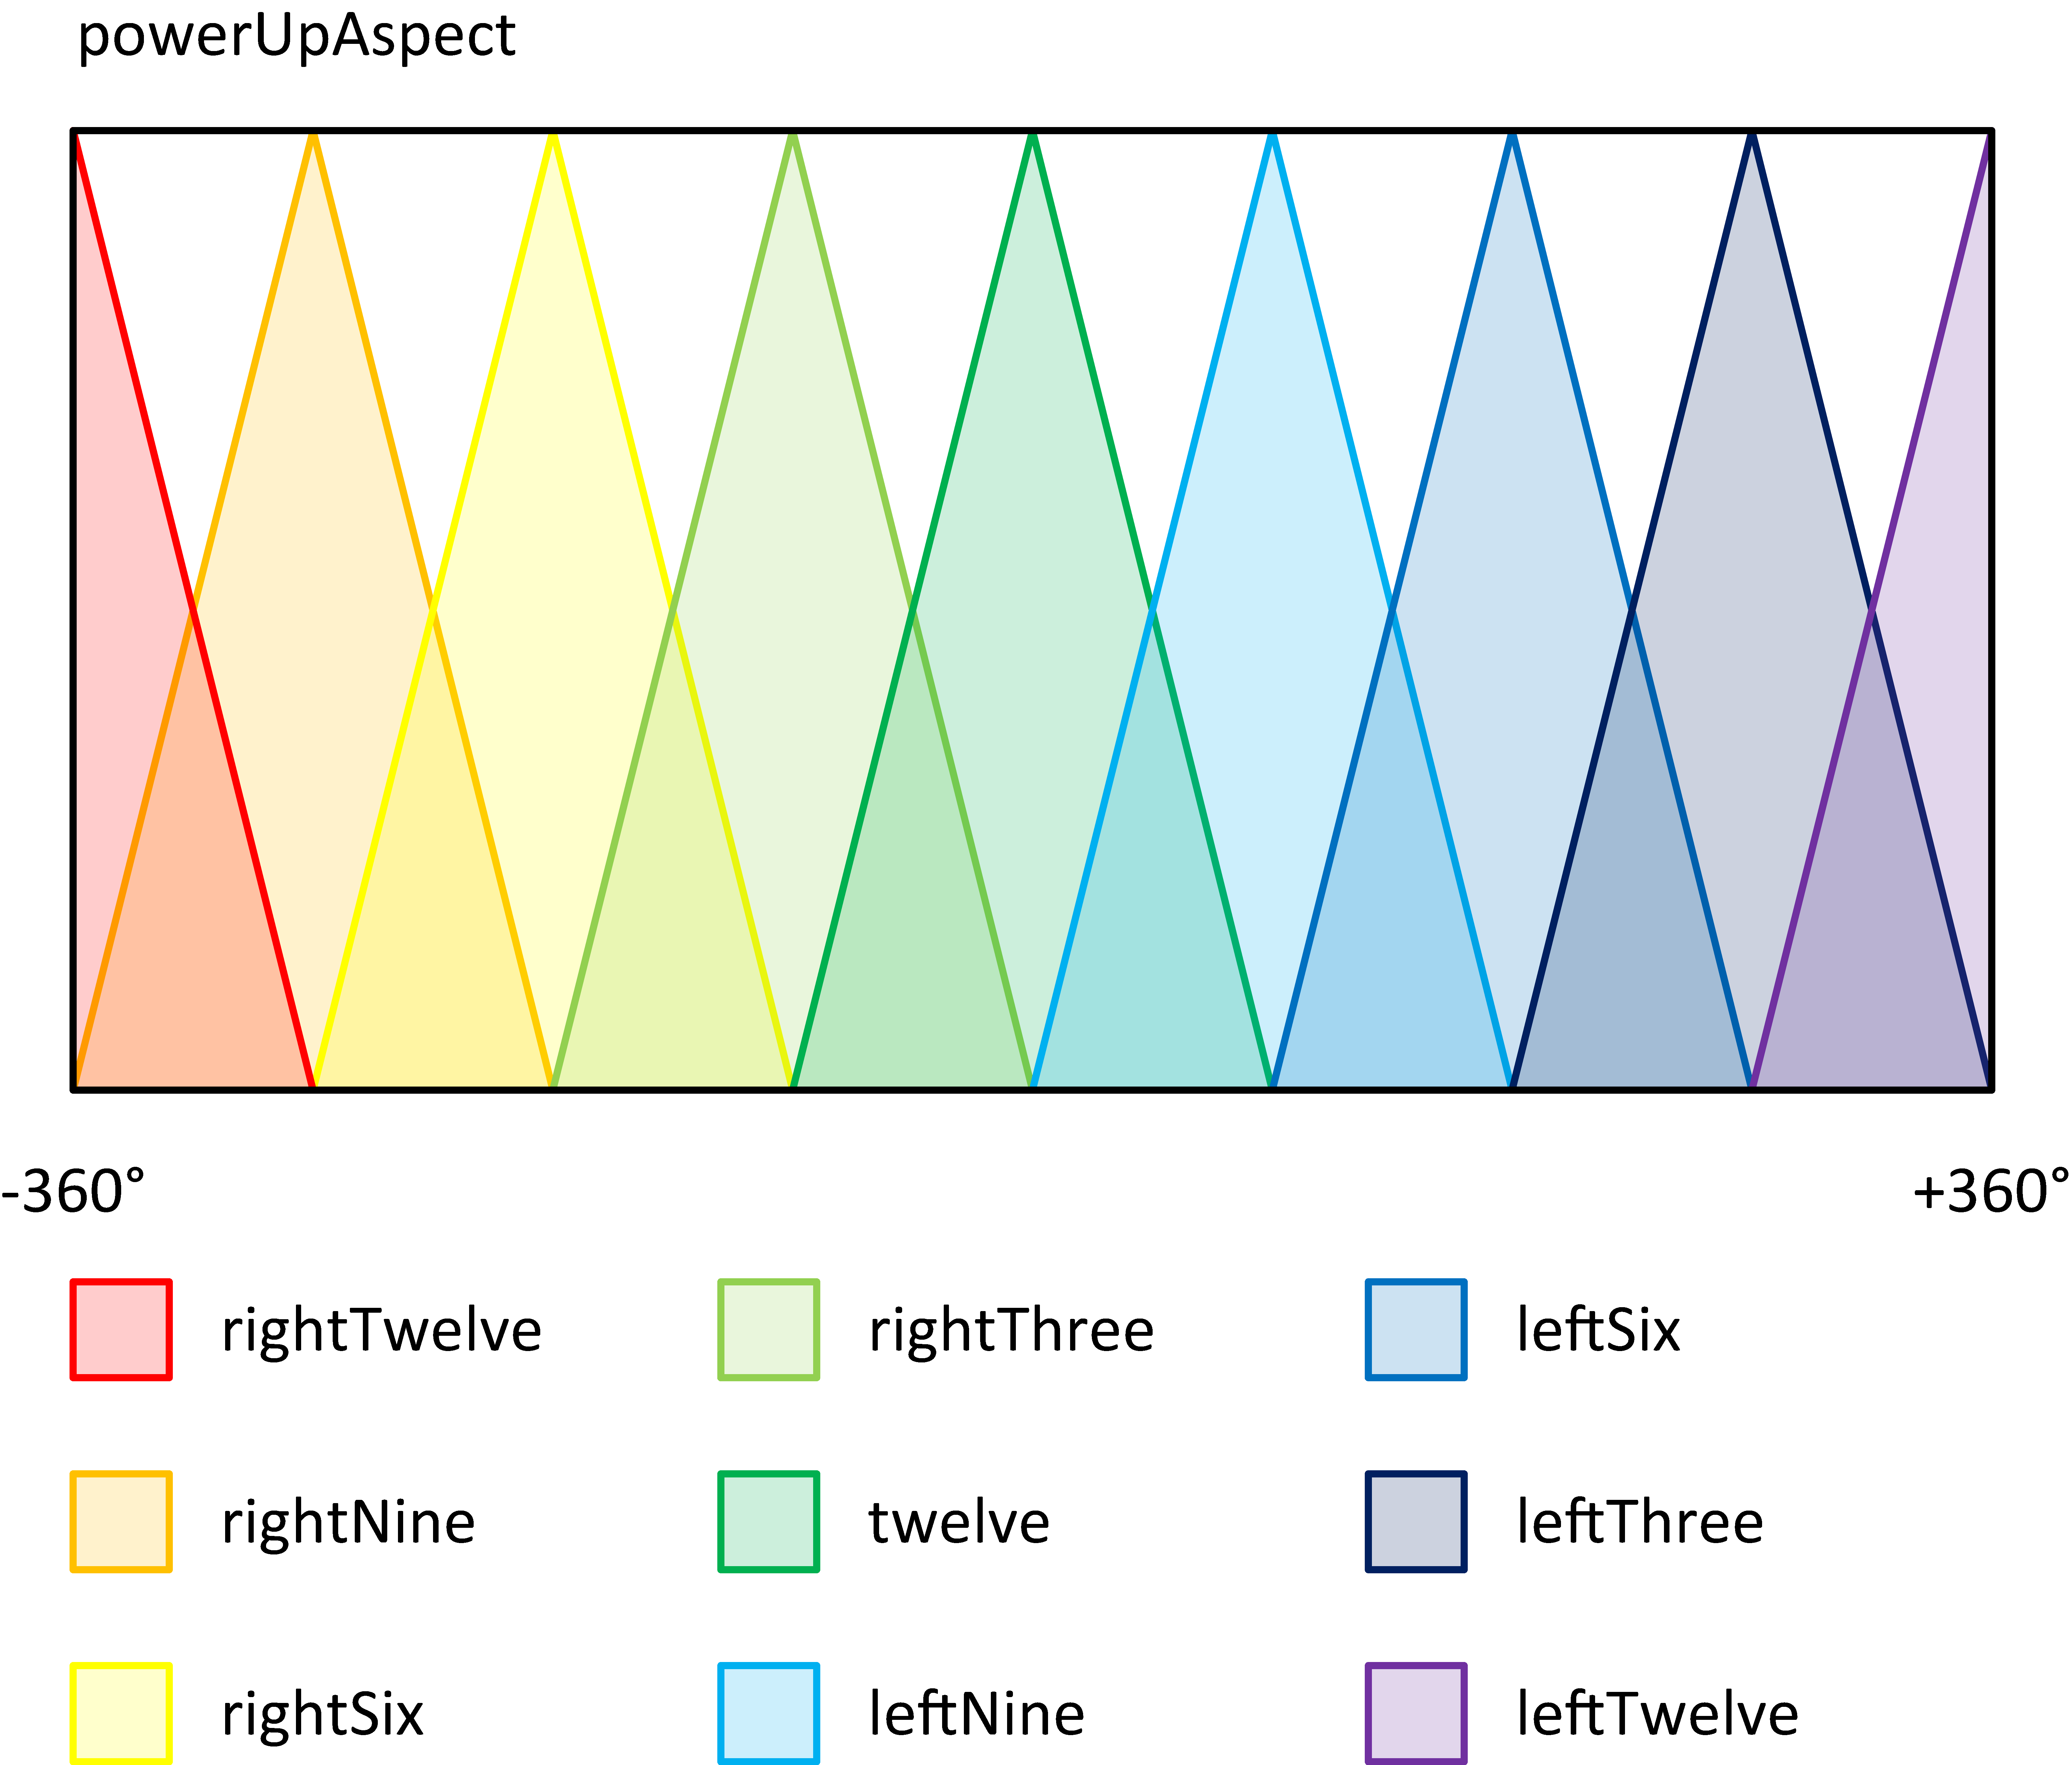
\includegraphics[scale=0.08]{./img/pdf/powerUpAspectSets.pdf}
\end{figure}

\section{Output linguistic variables}

Due to the fact that the fuzzy logic API does not provide a method to prioritize rules, defensive and offensive versions of some output linguistic variables have been defined. Boolean variables are defined, which are then tested to determine which version of the rule is fired, during a given situation.

For example, the defensive turn rule only considers the blast linguistic variables as input, whereas the offensive turn rule considers both target and blast linguistic variables.

\subsection{Defensive rules}

\subsubsection{defensiveTurn}

The \emph{defensiveTurn} linguistic variable defines which heading the saucer will take, in degrees, according to the rules that govern defensive turning. The linguistic variables used as input for \emph{defensiveTurn} are: \mintinline{console}{layerVar = blastDist}, \\ \mintinline{console}{rowVar = blastAngleOff}, and \mintinline{console}{colVar = blastAspect}, creating a 3D rule matrix. Note that \emph{r} and \emph{l} represent right and left in the table.
\\
\\
For example: IF (close) AND (rightSix) AND (zero) THEN (-90) \\
In other words, IF the energy blast is close, AND it is behind the player, AND it's heading towards the player, THEN turn right for 90$^{\circ}$.

\begin{table}[H]
\centering
\caption{\emph{defensiveTurn} \emph{close}}
\label{Turn rule table}
\begin{tabular}{r|r|r|r|r|r|r|r|r|r}
 		& rTwelve 	& rNine 	& rSix 		& rThree 		& twelve 	& lNine 	& lSix 		& lThree	& lTwelve		\\ \hline
rZero	& 0			& 0			& -90		& 0 		 	& 0			& 0			& +90	 	& 0			& 0				\\
r270	& +90		& 0			& 0			& +180			& +90		& 0			& 0			& +180		& +90			\\
rMerge	& 0			& 0			& -90	 	& 0				& 0			& 0			& +90		& 0			& 0				\\
r90		& +90		& -180		& 0 		& 0				& -90		& -180		& 0			& 0			& +90			\\
zero 	& 0			& 0 		& -90 		& 0				& 0			& 0			& +90		& 0			& 0				\\
l90 	& -90		& 0 		& 0			& +180			& +90		& 0			& 0			& +180		& -90			\\
lMerge	& 0			& 0 		& -90 		& 0				& 0			& 0			& +90		& 0			& 0				\\
l270 	& -90		& -180 		& 0			& 0				& -90		& -180		& 0			& 0			& -90			\\
lZero 	& 0			& 0 		& -90	 	& 0				& 0			& 0  		& +90		& 0			& 0				\\
\end{tabular}
\end{table}

\begin{table}[H]
\centering
\caption{\emph{defensiveTurn} \emph{far}}
\label{Turn rule table}
\begin{tabular}{r|r|r|r|r|r|r|r|r|r}
 		& rTwelve 	& rNine 	& rSix 		& rThree 	& twelve 	& lNine 	& lSix 		& lThree	& lTwelve	\\ \hline
rZero	& 0			& 0			& 0			& 0 	 	& 0			& 0			& 0	 		& 0			& 0			\\
r270	& 0			& 0			& 0			& 0			& 0			& 0			& 0			& 0			& 0			\\
rMerge	& 0			& 0			& 0	 		& 0			& 0			& 0			& 0			& 0			& 0			\\
r90		& 0			& 0			& 0 		& 0			& 0			& 0			& 0			& 0			& 0			\\
zero 	& 0			& 0 		& 0	 		& 0			& 0			& 0			& 0			& 0			& 0			\\
l90 	& 0			& 0 		& 0			& 0			& 0			& 0			& 0			& 0			& 0			\\
lMerge	& 0			& 0 		& 0	 		& 0			& 0			& 0			& 0			& 0			& 0			\\
l270 	& 0			& 0	 		& 0 		& 0			& 0			& 0			& 0			& 0			& 0			\\
lZero 	& 0			& 0 		& 0	 		& 0			& 0			& 0  		& 0			& 0			& 0			\\
\end{tabular}
\end{table}

The far rules have zero values so that the player does not react and maintains current heading when the energy blast is far, and is not a threat.

\subsubsection{defensiveSpeed}

The \emph{defensiveSpeed} linguistic variable defines how fast the saucer will travel, according to the rules that govern defensive speed. The linguistic variables used for input for \emph{defensiveSpeed} are: \mintinline{console}{layerVar = blastDist}, \mintinline{console}{rowVar = blastAngleOff}, and \mintinline{console}{colVar = blastAspect}, creating a 3D rule matrix.
\\
\\
For example: IF (close) AND (rightSix) AND (zero) THEN (125) \\
In other words, IF the energy blast is close, AND it is behind the player, AND it's heading towards the player, THEN speed is 125.

\begin{table}[H]
\centering
\caption{\emph{defensiveSpeed} \emph{close}}
\label{Turn rule table}
\begin{tabular}{r|r|r|r|r|r|r|r|r|r}
 		& rTwelve 	& rNine 	& rSix 		& rThree 		& twelve 	& lNine 	& lSix 		& lThree	& lTwelve		\\ \hline
rZero	& 50		& 125		& 125		& 125 		 	& 50		& 125		& 125 		& 125		& 50			\\
r270	& 50		& 125		& 50		& 125			& 50		& 125		& 50		& 125		& 50			\\
rMerge	& 50		& 125		& 50	 	& 125			& 125		& 125		& 50		& 125		& 50			\\
r90		& 50		& 125		& 50 		& 125			& 125		& 125		& 50		& 125		& 50			\\
zero 	& 50		& 125 		& 125 		& 125			& 50		& 125		& 125		& 125		& 50			\\
l90 	& 50		& 125 		& 50		& 125			& 125		& 125		& 50		& 125		& 50			\\
lMerge	& 50		& 125 		& 50	 	& 125			& 125		& 125		& 50		& 125		& 50			\\
l270 	& 50		& 125	 	& 50 		& 125			& 50		& 125		& 50		& 125		& 50			\\
lZero 	& 50		& 125 		& 125	 	& 125			& 50		& 125  		& 125		& 125		& 50			\\
\end{tabular}
\end{table}

\begin{table}[H]
\centering
\caption{\emph{defensiveSpeed} \emph{far}}
\label{Turn rule table}
\begin{tabular}{r|r|r|r|r|r|r|r|r|r}
 		& rTwelve 	& rNine 	& rSix 		& rThree 		& twelve 	& lNine 	& lSix 		& lThree	& lTwelve		\\ \hline
rZero	& 50		& 50		& 75		& 50 		 	& 50		& 50		& 75 		& 50		& 50			\\
r270	& 50		& 50		& 50		& 75			& 50		& 50		& 50		& 75		& 50			\\
rMerge	& 50		& 50		& 50	 	& 50			& 75		& 50		& 50		& 50		& 50			\\
r90		& 50		& 75		& 50 		& 50			& 75		& 75		& 50		& 50		& 50			\\
zero 	& 50		& 50 		& 75 		& 50			& 50		& 50		& 75		& 50		& 50			\\
l90 	& 50		& 50 		& 50		& 75			& 75		& 50		& 50		& 75		& 50			\\
lMerge	& 50		& 50 		& 50	 	& 50			& 75		& 50		& 50		& 50		& 50			\\
l270 	& 50		& 75	 	& 50 		& 50			& 50		& 75		& 50		& 50		& 50			\\
lZero 	& 50		& 50 		& 75	 	& 50			& 50		& 50  		& 75		& 50		& 50			\\
\end{tabular}
\end{table}

\subsection{Offensive rules}

\subsection{Neutral}

\subsubsection{getPowerTurn}


\newpage

\section{Sample fuzzy rule}

\subsection{Turning rule}

This section will examine the implementation of the fuzzy rules that govern the saucer's ability to turn, and will use the following situation, as shown in Figure 4 to demonstrate how the \emph{turn} output rules are fired:

\begin{figure}[H]
\centering
\caption{Sample game screen}
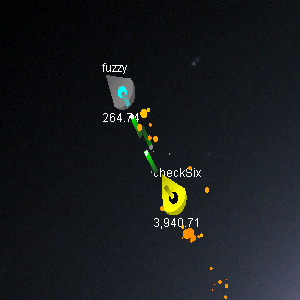
\includegraphics[scale=1]{./img/png/gameScreen.png}
\end{figure}

The yellow saucer in Figure 4 is the \emph{player}, called \emph{checkSix}, while the enemy is the grey saucer, called \emph{fuzzy}. Note that \emph{fuzzy} is controlled with the original, existing fuzzy controller supplied with the assignment. Two \emph{turn} rules are fired during this sequence:

\begin{itemize}
	\item Rule 1:
		\begin{itemize}
			\item IF (\emph{heading angle} IS front) AND (\emph{energy difference} IS winning) THEN (\emph{turn} IS 0)
		\end{itemize}	 
	\item Rule 2:
		\begin{itemize}
			\item IF (\emph{heading angle} IS left front) AND (\emph{energy difference} IS winning) THEN (\emph{turn} IS 90)
		\end{itemize}
\end{itemize}

\subsubsection{\emph{Energy difference} antecedent}

\emph{Energy difference} will be explored first, since the value is the same in both instances of Rule 1 and Rule 2 above. The \emph{energy difference} antecedent, which in this case is \emph{winning}, is demonstrated by the difference of energy between the two saucers. \emph{checkSix} has 3940.71 joules of energy remaining, while \emph{fuzzy} only has 264.74. The \emph{energy difference} is +3675.97j. Therefore, \emph{checkSix} is \emph{winning}. Figure 5 below demonstrates the firing of this antecedent, and shows that the fuzzy set value is +3675.97, while $\mu$, the membership value to the \emph{winning} fuzzy set, is 1.

\begin{figure}[H]
\centering
\caption{\emph{Energy difference} antecedent}
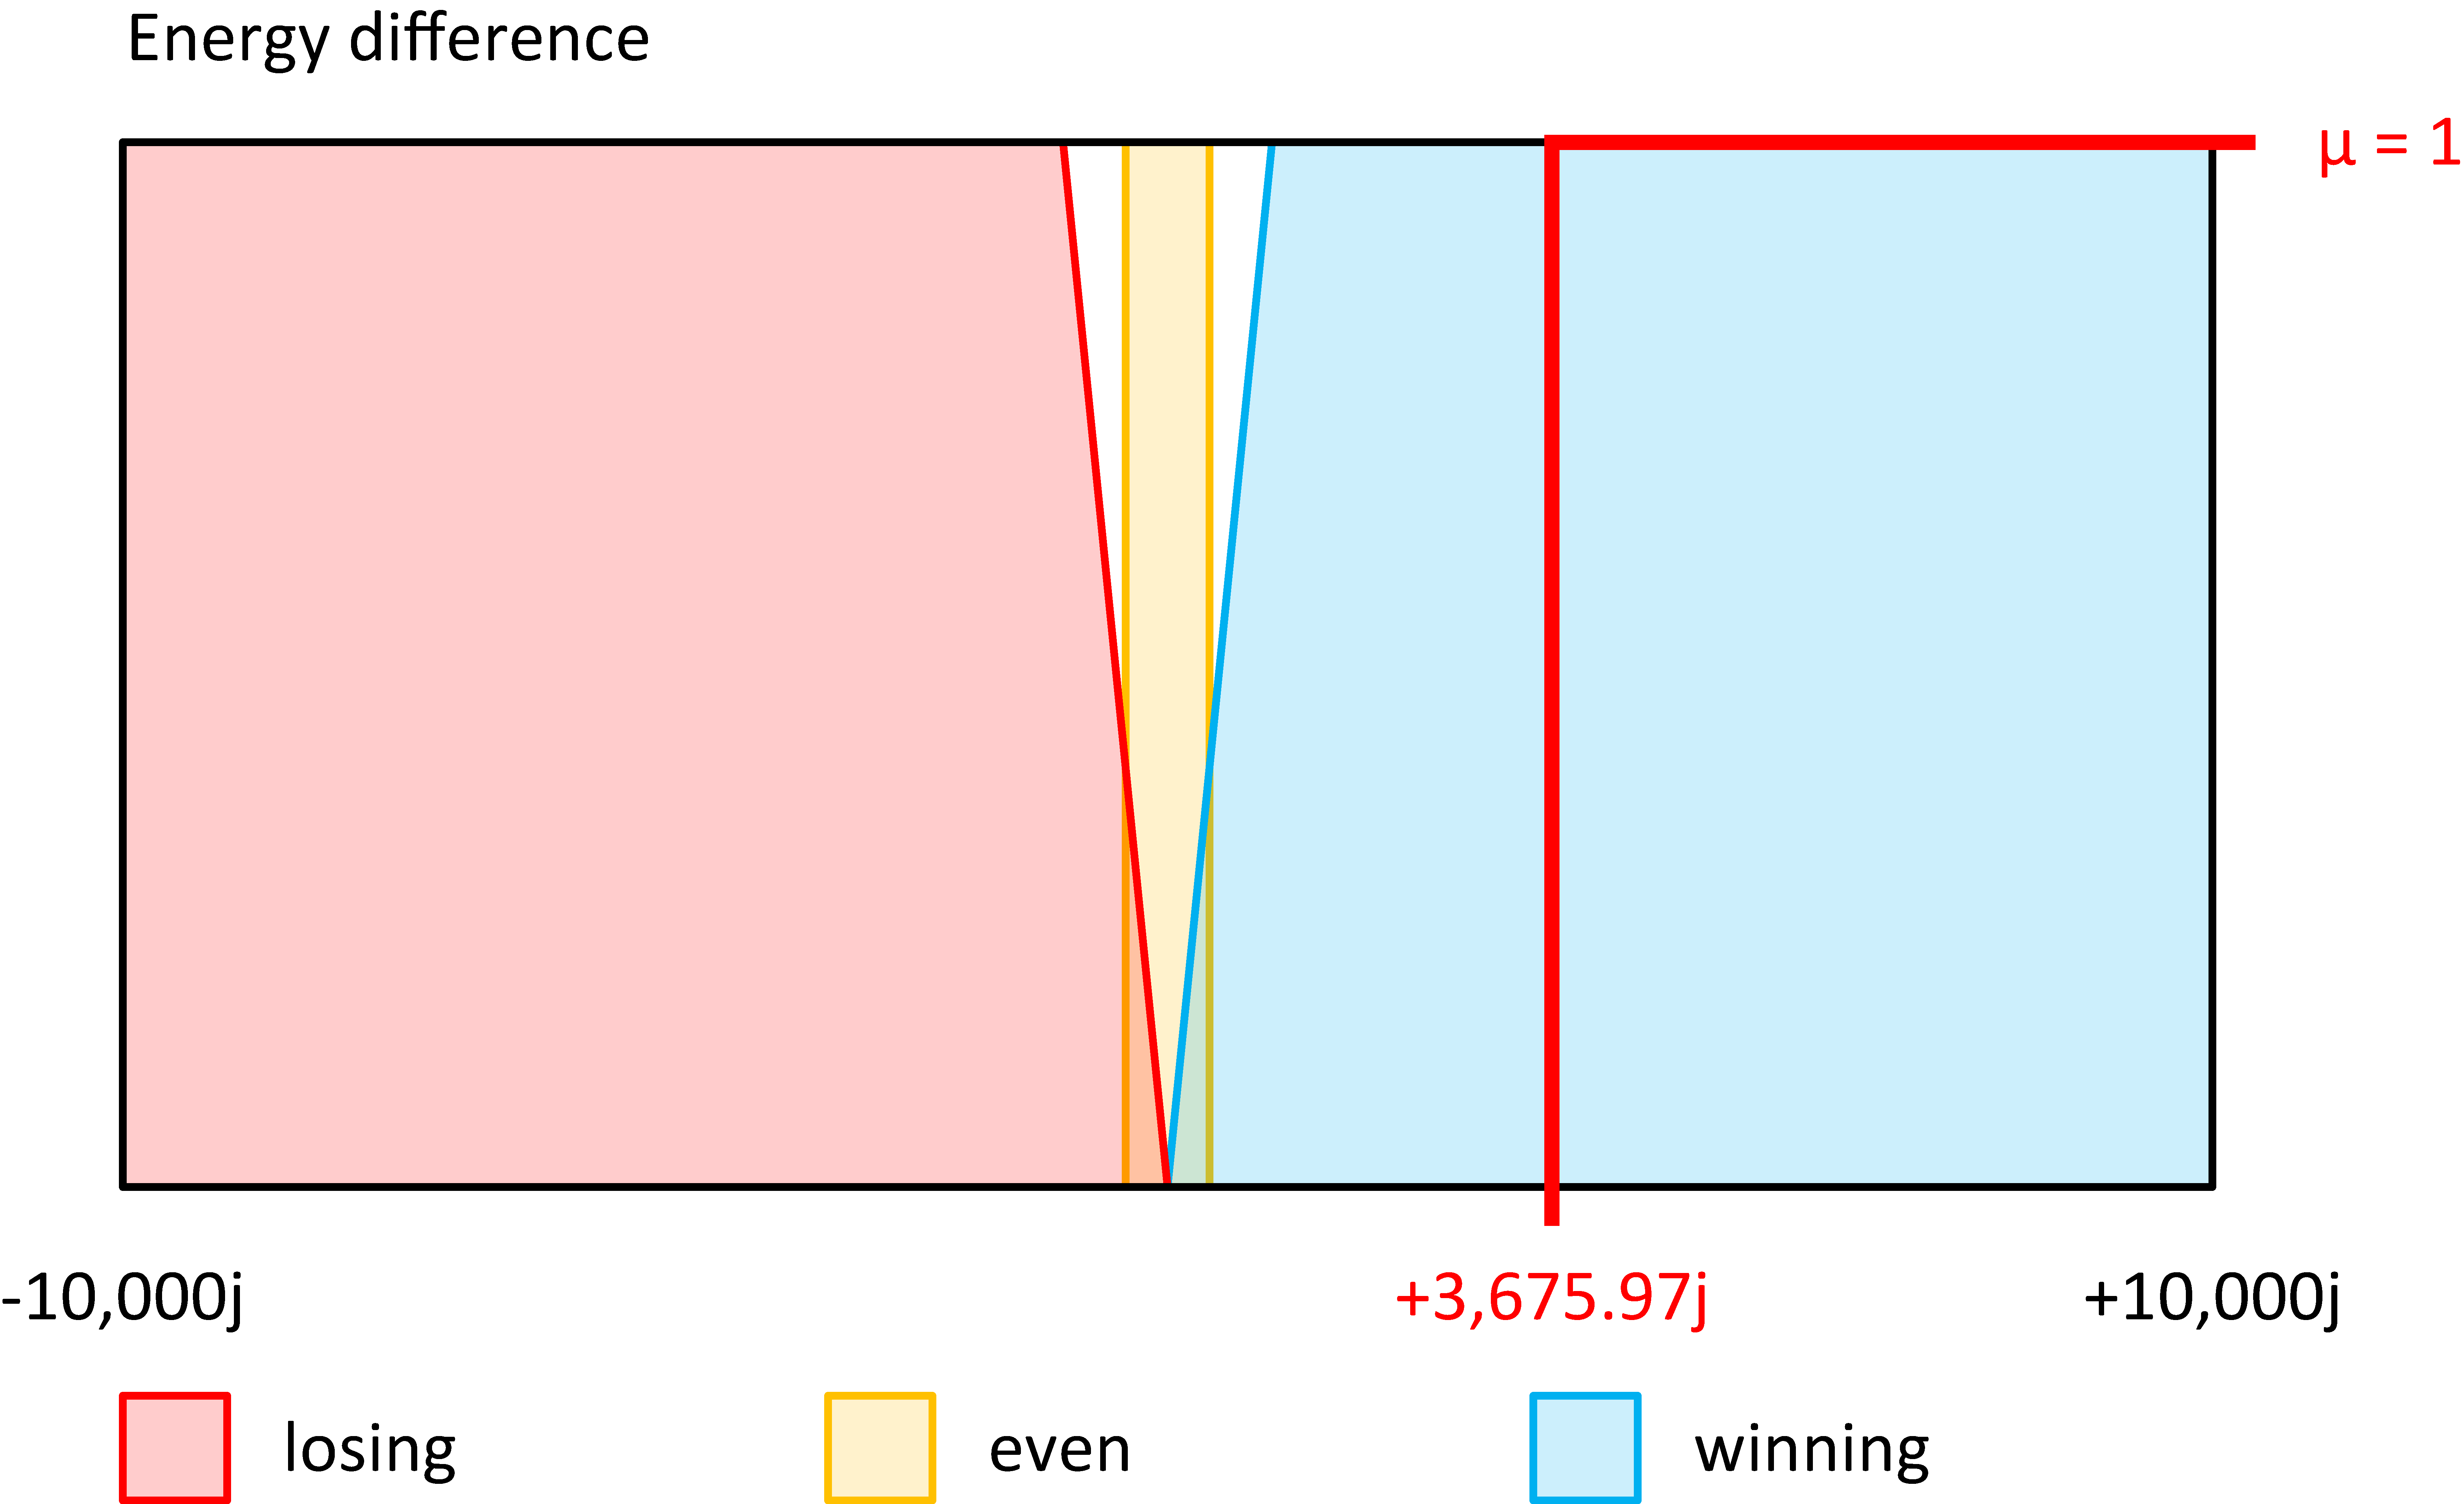
\includegraphics[scale=0.1]{./img/pdf/turnRule_energyDiff.pdf}
\end{figure}

\subsubsection{\emph{Heading angle} antecedent}

\emph{Heading angle} causes Rule 1 and Rule 2 to fire, with \emph{front} and \emph{leftFront}. This is due to the configuration of the two fuzzy sets. As seen previously in Figure 3, the \emph{leftFront} fuzzy set begins at 50\% of the \emph{front} fuzzy set range. In other words, any value higher than the median value of \emph{front} will also belong to the \emph{leftFront} set. Conversely, any value lower than the median value of \emph{front} will also belong to the \emph{rightFront} set. Figure 6 below demonstrates the firing of these two antecedents, their fuzzy set values and their $\mu$ values.

\begin{figure}[H]
\centering
\caption{\emph{Heading angle} antecedent}
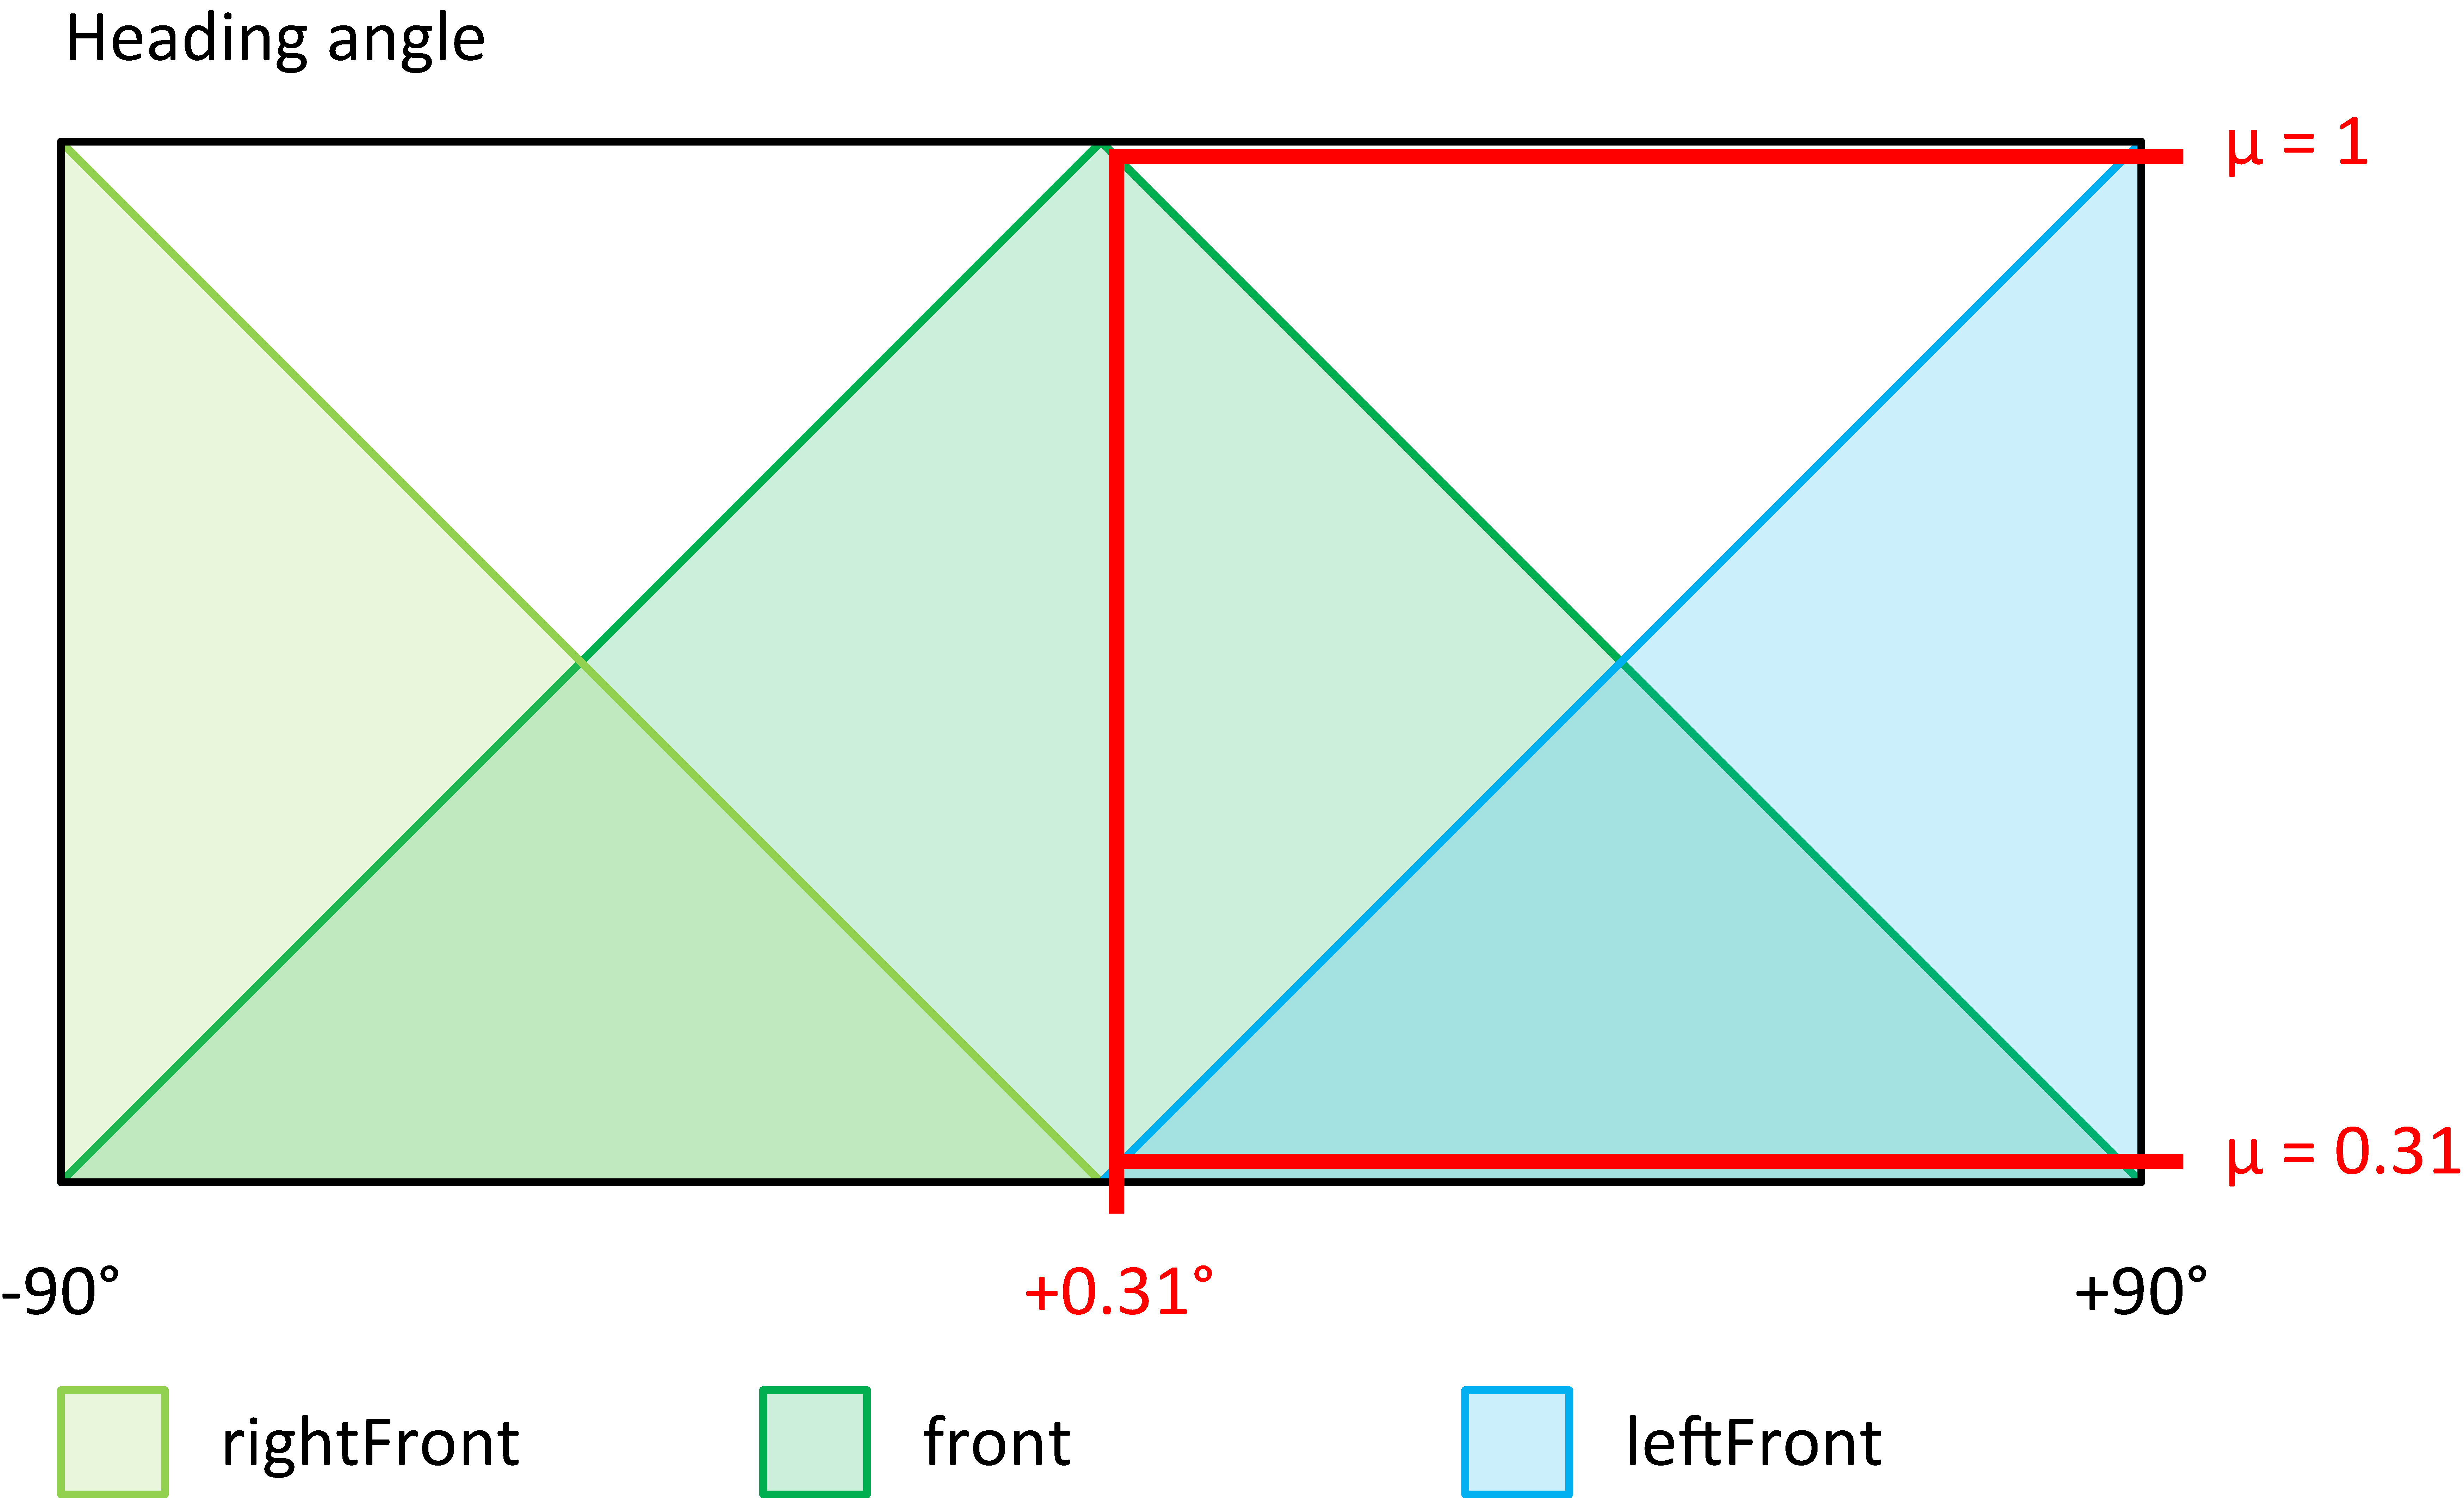
\includegraphics[scale=0.1]{./img/pdf/turnRule_headingAngle.pdf}
\end{figure}

Figure 6 shows a simplified view of the \emph{heading angle} sets, only displaying -90$^{\circ}$ to +90$^{\circ}$ during the firing of Rule 1 and Rule 2. The \emph{heading angle} value of +0.31$^{\circ}$ belongs to the \emph{front} fuzzy set at $\mu$ = 1, and also belongs to the \emph{leftFront} fuzzy set at $\mu$ = 0.31, hence the firing of the two rules, thus providing two inputs. These inputs, along with the \emph{energy difference} input will be aggregated to create a single, crisp output, as explained in the next section.

\subsubsection{Rule aggregation}

When multiple inputs are provided by the same antecedent, as seen in Section 4.1.2, Sugeno style inference calculates the weighted average to provide a single, crisp input, using the following formula:

{\LARGE
	\begin{align}
	\mbox{MA} = \frac{\sum^N_{i=1} \mu(k_i) k_i}{\sum^N_{i=1} k_i}
	\end{align}
}

\noindent
Therefore, to calculate the weighted average for the two \emph{heading angle} inputs for the example shown in Figure 6:

{\LARGE
	\begin{align}
	\mbox{MA} &= \frac{1 \times 0.31 + 0.31 \times 0.31}{1 + 0.31} \\
	&= 0.31
	\end{align}
}

\noindent
Subsequently, the crisp output from the two \emph{heading angle} antecedents is 0.31. However, $\mu$ for the \emph{energy difference} antecedent must also be considered. As discussed in Section 4.1.1, $\mu$ = 1 for \emph{energy difference}.

Since the example rule performs an AND operation between the two antecedents, fuzzy set operations dictate that an intersection operation must occur to determine the final, crisp output. Therefore, the following function is appropriate:

{\LARGE
	\begin{align}
	\mbox{output} = \mbox{min}(\mu(k_1), \mu(k_2), \mbox{...}, \mu(k_n))
	\end{align}
}

\noindent
When applied to our example rules that have been fired:

{\LARGE
	\begin{align}
	\mbox{output} &= \mbox{min}(1, 0.31) \\
	&= 0.31
	\end{align}
}

\noindent
Therefore, the final, crisp output for the example scenario is a turn of 0.31$^{\circ}$. In other words, from its current direction of 0.0$^{\circ}$, the saucer will turn LEFT for 0.31$^{\circ}$, in order to follow the enemy, who is in front, and slightly to the left.
\newpage

\section{Learnings}

Although I believe I have a firm grasp on the basic concepts of fuzzy logic, I had a considerable amount of trouble understanding the logic behind \emph{turning} the saucer. I ran several tests, printing the opponent direction values during runtime to understand the relationship between where the player saucer is, and where the enemy is, and the values that were returned each frame. It was only until I imagined that the negative, right-hand turn values as ``turning counter-clockwise'' did I manage to tune the turn rules to a working manner.

My initial concept was to aggressively attack the opponent as soon as the game started, which worked fine. However, I could not test my defensive strategy, and initially just hoped that my saucer would immediately overcome the enemy with firepower and always be within the ``winning'' fuzzy set limits. Eventually, I realised that the original \mintinline{console}{FuzzyController.java} class could be made more difficult by changing the values, as listed below:

\begin{listing}[H]
\caption{FuzzyController.java modifications}

\begin{javacode}
public FuzzyController() throws Fuzzy Exception {
  // ...
  final double maxPower = Saucer.MAX_POWER;
  final double midPower = maxPower; // originally divided by 5.0
  final double lowPower = maxPower; // originall divided by 20.0
  // ...
}
\end{javacode}
\end{listing}

In doing so, the opponent always fires at maximum power when close, testing whether or not my offensive strategy to always stay right next to the enemy worked. Initial tests proved that my strategy did not work and was destroyed immediately. I needed to develop a substantial defensive strategy.

The heading angle fuzzy sets were modified from my original, arbitrarily chosen sets, to sets that are based on clock positions in relation to the player's position, similar to what a fighter pilot might say during combat, ie. ``Bandit at my six o'clock'', or ``Bogey at my nine''. The turn output spikes were also chosen based on the clock analogy, resulting in much more controlled behaviour, and enabled me to define a defensive strategy through the turn rules.

However, the rules require refinement, as confusion can occur when the player saucer hits a battle space border and the opponent direction being returned switches between negative and positive values. This confusion results in the player saucer spinning on the spot, and would be a major problem if turns cost energy. Firepower could also be improved by refining input sets or rules. Currently, the player saucer may fire weak shots even though the enemy is far away, resulting in wasted energy.

My offensive strategy is also far from perfect and has much room for improvement. Sitting right behind the enemy and giving chase during offence may suit well to space/aircraft with fixed, forward facing armament, but is a dangerous place to be when the enemy can rotate his weapon to face the rear.
\newpage

\section{Conclusion}

This report examined the application of fuzzy logic using Sugeno style inference in a video game. The video game involved developing a fuzzy logic controller, which controls an armed flying saucer with the sole purpose of destroying the enemy saucer.

The linguistic input variables and their fuzzy sets were explored, as well as the output variables and the associated rules. These rules governed the behaviour of the saucer and attempted to implement the two overall tactics developed for this assignment:

\begin{itemize}
	\item Commit to the battle and fly offensively when the score is even or if winning
	\item Disengage from the battle and fly defensively when losing
\end{itemize}

An example rule was examined, and the aggregation of a crisp output was explained, based on Sugeno style inference. Finally, learning experiences throughout the work of this assignment were discussed.

\subsection{Results}

The following tables on the final page display the results of tournaments between the \emph{checkSix} controller versus the \emph{simple} controller, \emph{fuzzy} controller, as well as the modified fuzzy controller, as discussed in Section 5. The modified fuzzy controller is referred to as \emph{fuzzyMaxPower} in the table. The average score over 10 battles per tournament is shown, with five consecutive tournaments executed per opponent.

\newpage

\begin{table}[H]
\centering
\caption{\emph{checkSix} vs. \emph{simple}}
\label{checkSix vs. simple}
\begin{tabular}{r|r|r}
Tournament	& checkSix	& simple	\\ \hline
1			& 3568.44	& 0.0		\\
2			& 3813.32	& 0.0		\\
3			& 3518.27	& 0.0		\\
4			& 3433.35	& 0.0		\\
5			& 3181.94	& 0.0
\end{tabular}
\end{table}

\begin{table}[H]
\centering
\caption{\emph{checkSix} vs. \emph{fuzzy}}
\label{checkSix vs. fuzzy}
\begin{tabular}{r|r|r}
Tournament	& checkSix	& fuzzy	\\ \hline
1			& 2586.32	& 0.0	\\
2			& 2709.84	& 0.0	\\
3			& 2652.23	& 0.0	\\
4			& 2245.64	& 0.0	\\
5			& 2769.11	& 0.0
\end{tabular}
\end{table}

\begin{table}[H]
\centering
\caption{\emph{checkSix} vs. \emph{fuzzyMaxPower}}
\label{checkSix vs. fuzzyMaxPower}
\begin{tabular}{r|r|r}
Tournament	& checkSix	& fuzzyMaxPower	\\ \hline
1			& 211.28	& 37.96			\\
2			& 125.43	& 26.95			\\
3			& 215.79	& 26.21			\\
4			& 108.29	& 13.24			\\
5			& 201.97	& 12.72
\end{tabular}
\end{table}

%\newpage
%\urlstyle{rm}
%\bibliographystyle{apacite}
%\addcontentsline{toc}{section}{References}
%\bibliography{./bib/Year_2-Sem_1-CSG2341-0b_A1}


\end{document}